\chapter{Architectural Design}
\label{ch:architectural-design}%

\section{Overview}
\label{sec:overview}%

\par The following is an overview of the BBP architecture general components. A more detailed view will be provided in
\ref{sec:deployment-view}.

\begin{figure}[H]
      \centering
      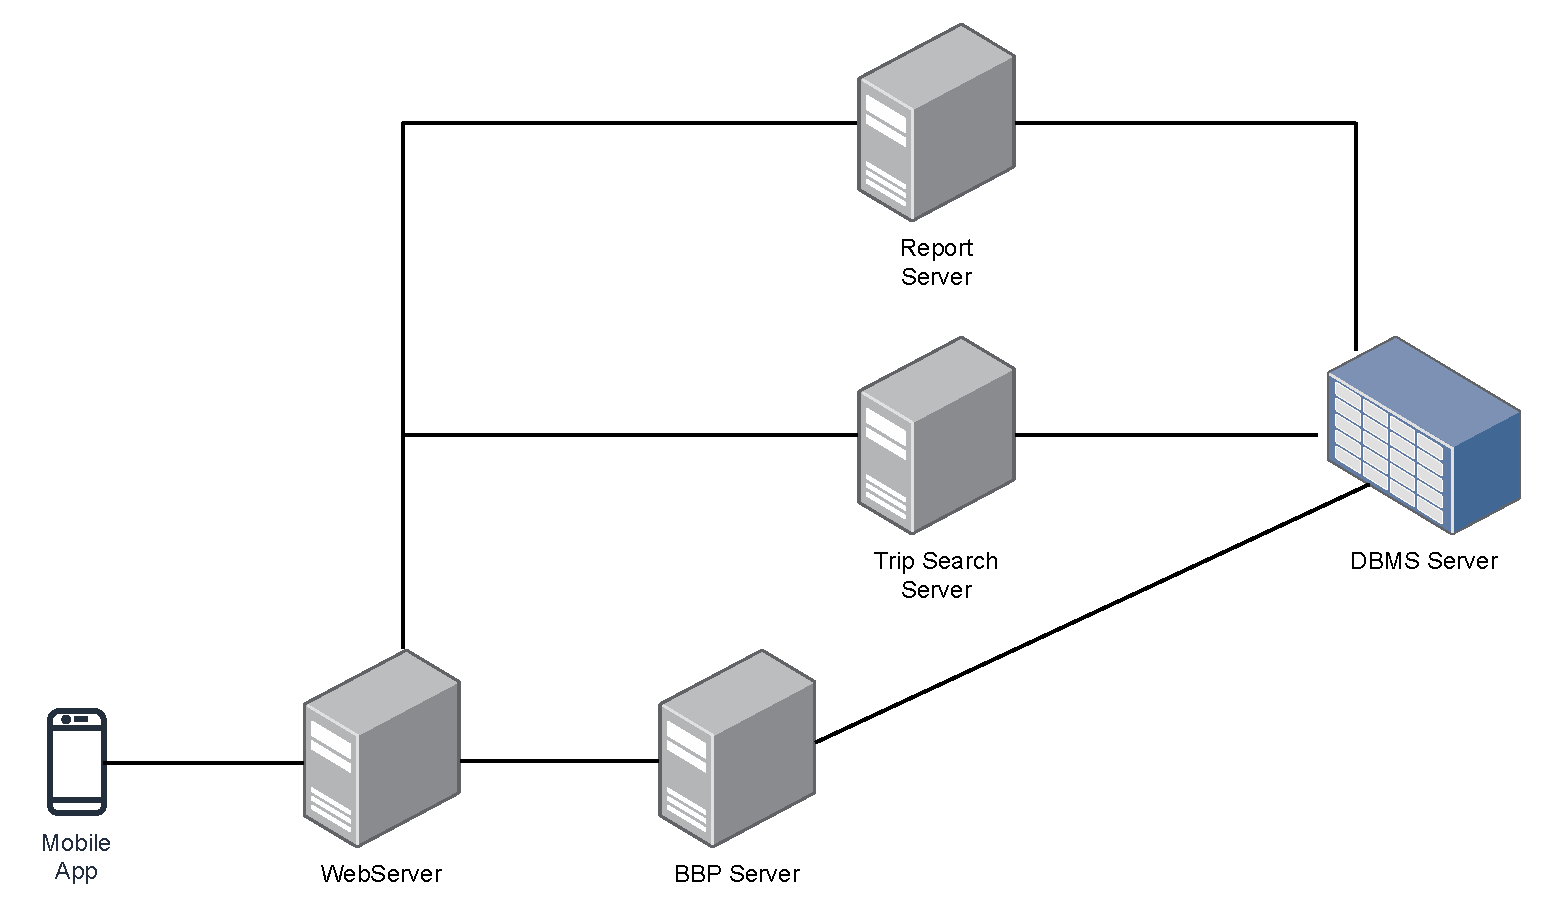
\includegraphics[width=1\textwidth]{Images/PDF/SysArchitetture.pdf}
      \caption{BBP Architecture Overview}
      \label{fig:overview}
\end{figure}

\par On the client side can be seen:
\begin{itemize}
      \item \textbf{Mobile App}: The application used by end users to record trips, either manually or automatically.
            The mobile app is responsible for accessing device sensors (e.g., GPS and motion sensors) and external
            services such as weather and map providers. Collected and enriched trip data is then sent to the backend
            for validation, storage, and aggregation.
\end{itemize}
\par On the server side, we can see:
\begin{itemize}
    \item \textbf{Web Server}: It handles HTTP/HTTPS communication between users and the BBP system. It acts as an API Gateway, serving the user interface and forwarding API requests to the core logical component, the BBP Server.
    \item \textbf{Trip Search Server}: A specialized server dedicated exclusively to handling path search operations. By receiving read-only requests directly from the Web Server and querying the DBMS, it offloads the main BBP Server, ensuring fast response times even during high traffic.
    \item \textbf{Report Server}: A dedicated server designed to handle crowd-sourced data submissions, such as manual obstacle reports. It operates independently from the high-bandwidth trip ingestion pipeline to process, validate, and persist discrete user feedback, ensuring that spikes in reporting activity do not interfere with real-time tracking performance.
    \item \textbf{BBP Server}: It represents the core backend of the system. It contains the main business logic and orchestrates the various sub-components dedicated to data and trip management. Internally, the logic is divided into the following functional modules:
    \begin{itemize}
        \item \textbf{Trip Search Service}: A specialized module dedicated to read operations. It receives search queries and efficiently queries the DBMS to retrieve paths and information.
        
        \item \textbf{Trip Ingestion Service}: The entry point of the writing pipeline. It is responsible for receiving and pre-processing raw telemetry data sent by user devices.
        
        \item \textbf{Trip Validation Service}: A processing component that analyzes data received from the Ingestion Service. Its task is to filter GPS errors, verify data consistency, and discard invalid anomalies before proceeding.
        
        \item \textbf{Trip Aggregation Service}: A critical component that receives validated data. It is responsible for merging the new trip information with the existing history for that road segment, updating the collective status of the path.
        
        \item \textbf{Trip Scoring Service}: The final step in the processing chain. It calculates or updates the quality "Score" of the path based on aggregated data and persists the final results into the DBMS.
    \end{itemize}
\end{itemize}

\section{Component View}
\label{sec:component-view}%

\subsection{High-Level Components}
\label{sub:high-level-components}%

\begin{figure}[H]
      \centering
      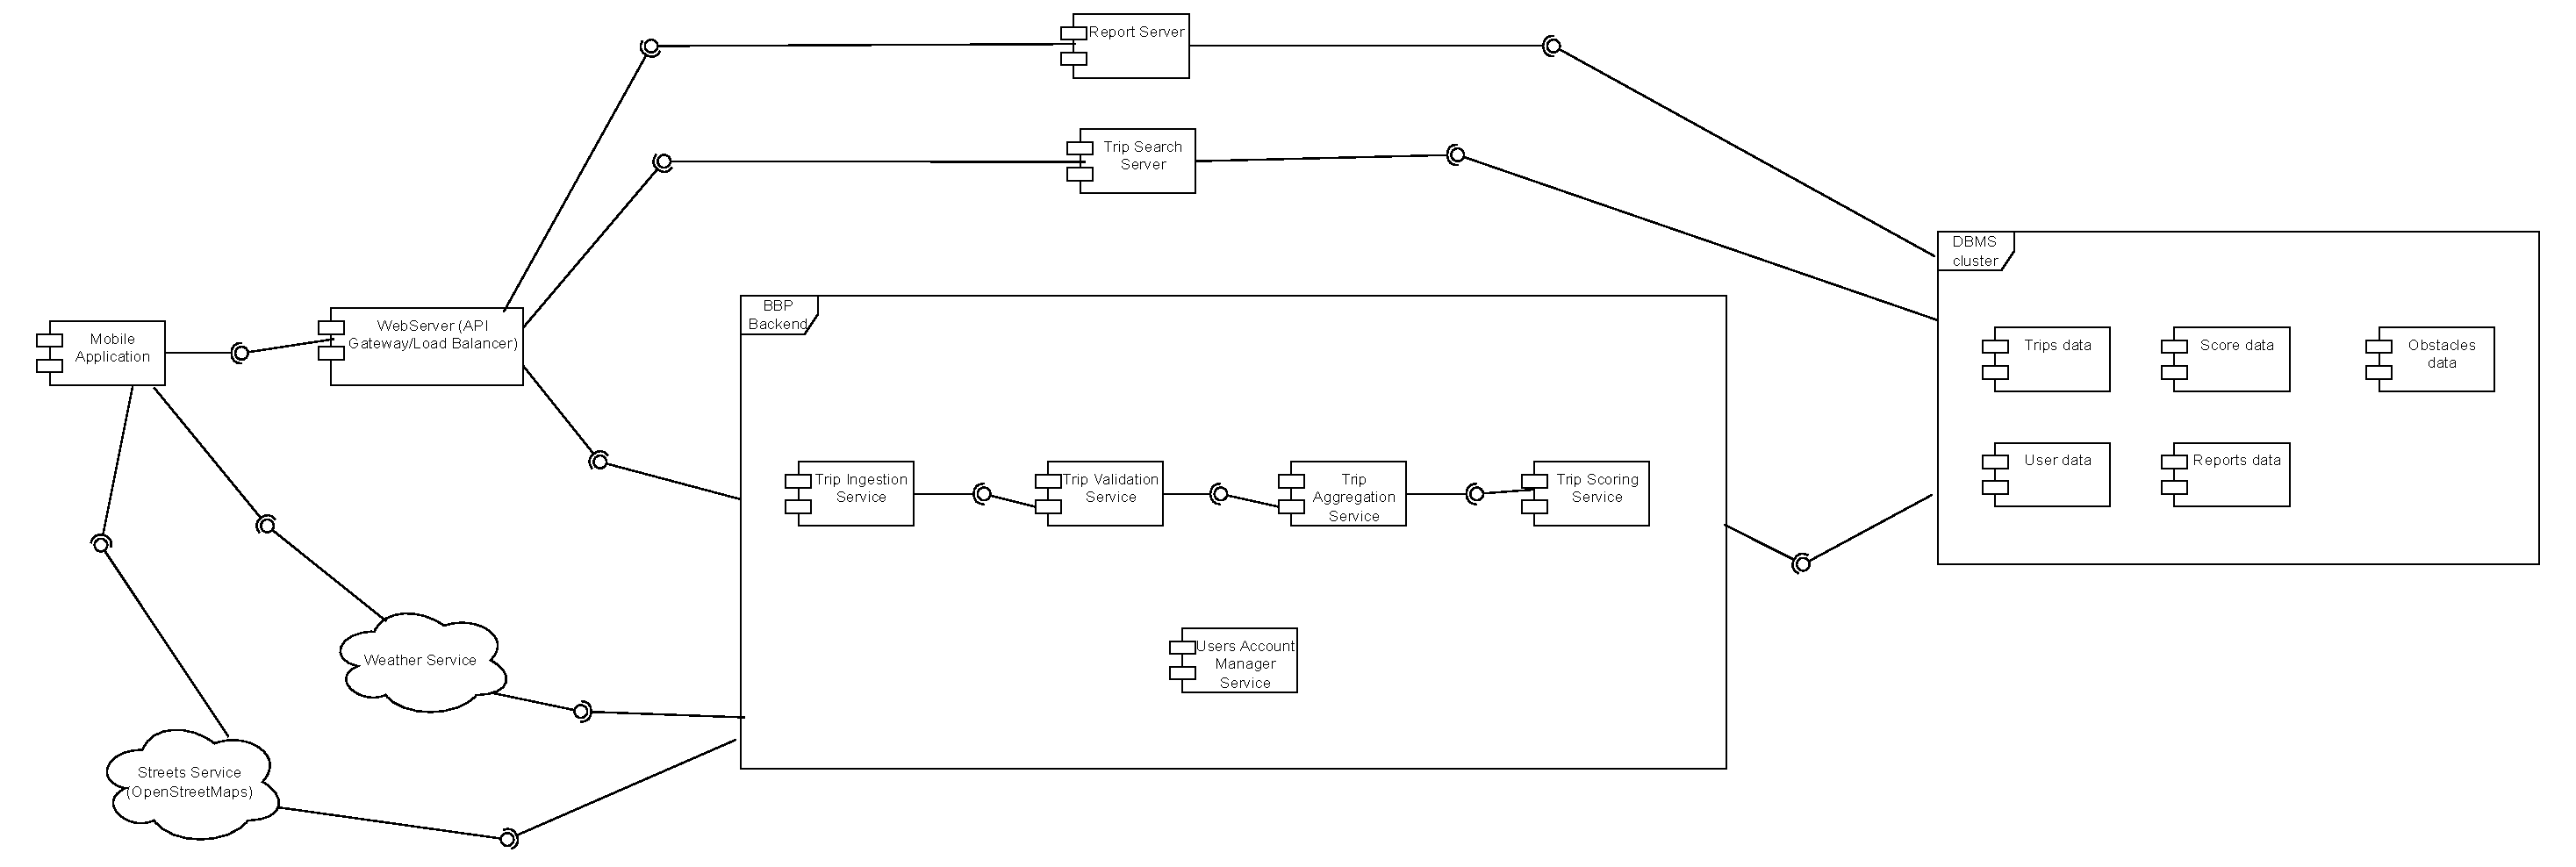
\includegraphics[width=1\textwidth]
      {Images/PDF/high level components.pdf}
      \caption{High-Level Components}
      \label{fig:high-level-components}
\end{figure}

\par Figure \ref{fig:high-level-components} shows the system architecture. It adopts a \textbf{Microservices} pattern to ensure modularity, scalability, and high availability. The components are organized into logical layers: Client, Entry Point, Backend Services, Data Persistence, and External Systems.

\subsubsection{Client Side}

\textbf{Mobile Application.}
The mobile application represents the primary interface for the end-user (Cyclist). It is responsible for acquiring high-frequency telemetry data, including GPS, accelerometer, and gyroscope measurements, directly from the device sensors. The application manages user interaction, map visualization, and initiates secure HTTPS requests toward the backend services. To preserve battery life and reduce computational overhead on the client device, it avoids heavy data processing, delegating these tasks entirely to the server-side infrastructure.

\subsubsection{Entry Point}

\textbf{WebServer (API Gateway / Load Balancer).}
The WebServer acts as the single entry point for the \textit{BBP Backend Cluster}, effectively decoupling the client from the internal microservices architecture. Its responsibilities include routing incoming requests to the appropriate backend service, such as forwarding path search requests to the \textit{Trip Search Service} or authentication requests to the \textit{Users Account Manager}. In addition, it performs load balancing by distributing incoming traffic across multiple active service instances to handle peak loads, and it manages security concerns by handling SSL termination and protecting internal endpoints from direct external access.

\subsubsection{Backend Services (BBP Backend Cluster)}

The backend is composed of independent microservices, each implementing a specific portion of the business logic and data processing pipeline.

\textbf{Users Account Manager Service.}
This service manages all logic related to user identity, including registration, authentication, and profile updates. It interacts exclusively with the \textit{User Data} storage to guarantee security and strict isolation of Personally Identifiable Information (PII).

\textbf{Trip Ingestion Service.}
The Trip Ingestion Service is a write-intensive component designed to receive raw telemetry streams from the mobile application. It acts as a high-throughput buffer to prevent data loss during periods of peak usage. Additionally, it interacts with the external \textit{Weather Service} to enrich incoming trip data with meteorological conditions at the time of recording.

\textbf{Trip Validation Service.}
This service is responsible for data quality assurance. It processes raw trip data to filter GPS inaccuracies and validate potential obstacles. To ensure spatial correctness, it queries the \textit{Streets Service (OpenStreetMap)} to perform map-matching operations, verifying that recorded coordinates correspond to actual physical roads.

\textbf{Trip Aggregation Service.}
The Trip Aggregation Service implements the collaborative logic of the system. It merges newly validated trip data with the historical state of bike paths and applies majority voting algorithms to resolve conflicting user reports, such as determining the effective roughness of a road segment.

\textbf{Trip Scoring Service.}
This service acts as the computation engine responsible for calculating the qualitative \textit{Score} of a path. It processes aggregated information, including surface smoothness, detected obstacles, and user ratings, to generate a numerical value representing the overall safety and quality of the route.
\subsubsection{Specialized Independent Servers}

To optimize resource allocation and ensure high availability, specific functionalities are hosted on dedicated server infrastructure, physically or logically separated from the core processing cluster. This architectural decision minimizes resource contention and isolates critical read/write workloads.

\textbf{Trip Search Server.}
Designed as a read-optimized component, this server implements the query side of the system's architecture (following a CQRS-like pattern). It is dedicated exclusively to handling user pathfinding queries by retrieving pre-calculated scores and obstacle data. By isolating this read-heavy workload on a dedicated server, the system ensures low-latency responses (under two seconds) regardless of the load on the write-intensive ingestion pipeline.

\textbf{Report Server.}
This server operates as an autonomous unit dedicated to handling crowd-sourced data submissions, such as manual obstacle reports or generic street feedback. Unlike the continuous telemetry stream processed by the Ingestion Service, user reports are discrete, asynchronous events. This server runs its own validation logic to filter spam or incorrect data before persisting validated reports into the central database, ensuring that spikes in user reporting do not interfere with the real-time tracking performance.


\subsubsection{Data Persistence Layer (DBMS Cluster)}

To support the heterogeneous requirements of the backend services, the data persistence layer is logically partitioned into a cluster of specialized data stores. The \textit{User Data} store maintains user profiles, credentials, and configuration settings, and is isolated to comply with privacy regulations such as GDPR. The \textit{Trips Data} store is optimized for time-series data and retains the large volume of raw telemetry streams collected from sensors. The \textit{Obstacles \& Reports Data} store contains validated obstacles, such as potholes and interruptions, as well as user-submitted reports. Finally, the \textit{Score Data} store holds the computed road quality scores and path statuses, and is optimized for fast spatial queries to efficiently support the \textit{Trip Search Service}.

\subsubsection{External Systems}

The architecture integrates with external systems to enhance the quality and reliability of the collected data. The \textit{Weather Service} is queried to enrich trip records with real-time meteorological context, such as rain and wind conditions. Additionally, the \textit{Streets Service (OpenStreetMap)} provides authoritative geospatial reference data used for coordinate validation and map-matching against existing road infrastructure.



\subsection{Low-Level Components}
\label{sub:low-level-components}%

\begin{figure}[H]
    \centering
    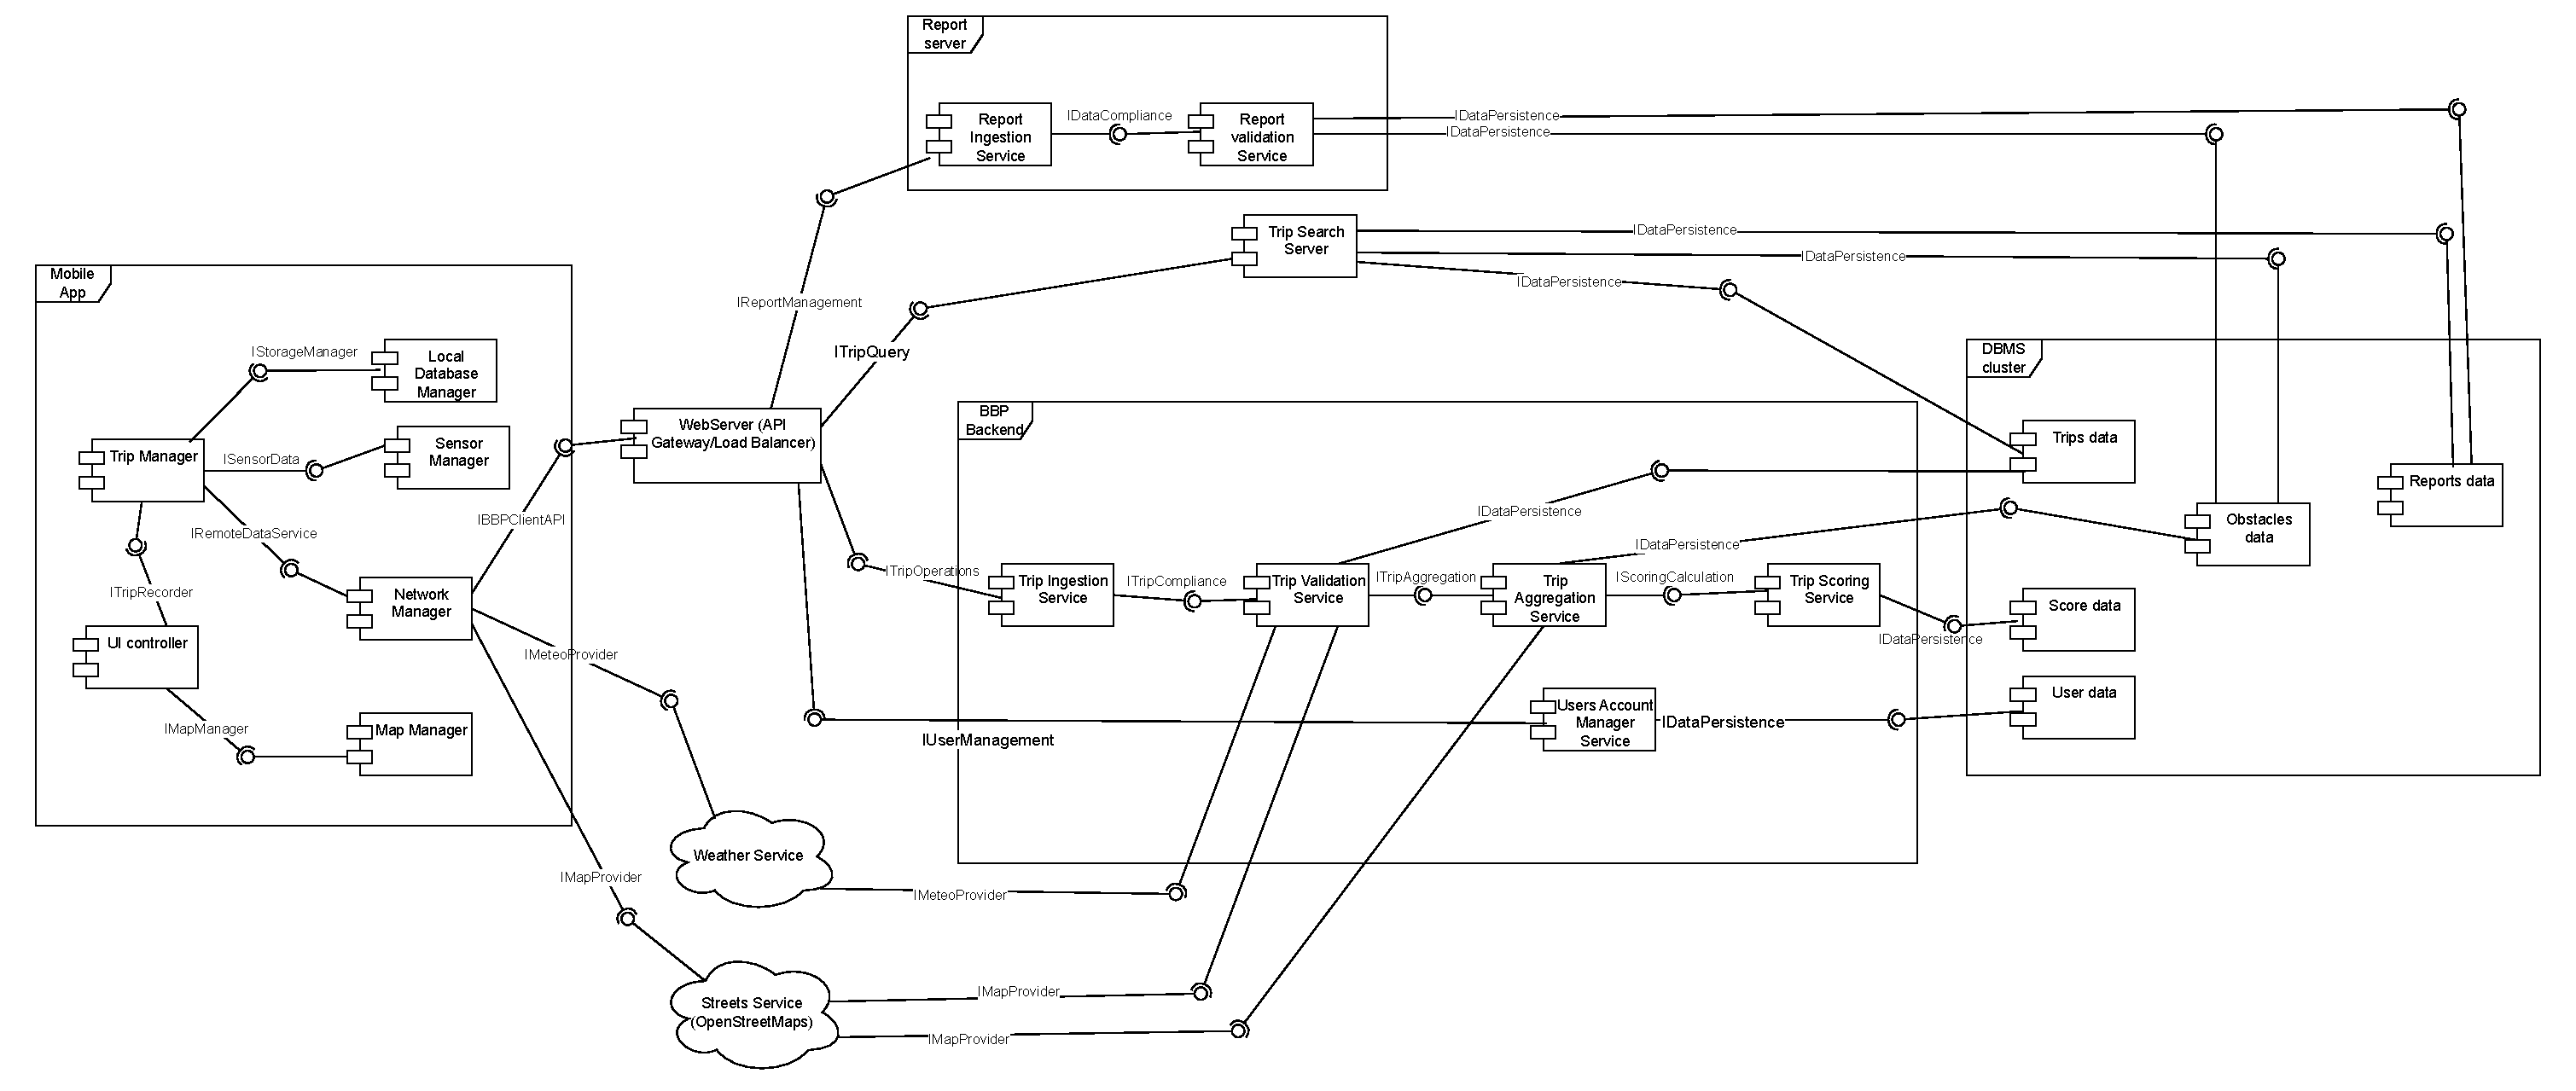
\includegraphics[
        width=1.1\textwidth,
        keepaspectratio
    ]{Images/PDF/low_level_comp.pdf}
    \caption{Low-Level Components}
    \label{fig:low-level-components}
\end{figure}
\subsubsection{Mobile Application Internal Components}

To ensure responsiveness, fault tolerance, and efficient resource usage, the Mobile Application is architected into distinct functional modules:

\textbf{UI Controller.}
This component manages the presentation layer of the application. It handles user interactions (e.g., starting a trip, submitting a report) and updates the visual interface based on the application state. It acts as the bridge between the user and the underlying logic components.

\textbf{Sensor Manager.}
A hardware abstraction layer responsible for interfacing with the device's physical sensors (GPS, Accelerometer, Gyroscope). It configures the sampling rate to balance data precision with battery consumption and provides a normalized stream of raw telemetry data to the Trip Manager.

\textbf{Trip Manager.}
This component acts as the central orchestrator for the tracking session. It manages the lifecycle of a trip (Start, Pause, Stop) and coordinates the flow of data. It receives raw readings from the Sensor Manager and directs them to the storage layer, ensuring no data is lost even if the network is unavailable.

\textbf{Local Database Manager.}
This component ensures data persistence and fault tolerance. It manages a local embedded database (e.g., SQLite) acting as a buffer. During a trip, data is written here first; this guarantees that if the application crashes or network connectivity is lost, the recorded telemetry is preserved and can be synchronized later.

\textbf{Network Manager.}
Responsible for all asynchronous communication with the backend services. It retrieves pending data from the Local Database Manager and handles the upload process to the \textit{Trip Ingestion Service} or \textit{Report Server}. It implements retry policies and data synchronization logic to handle intermittent network conditions transparently.

\textbf{Map Manager.}
This component wraps the mapping SDK (e.g., Google Maps or OSMdroid). It is responsible for rendering the map interface, drawing the user's current route, and visualizing map markers such as obstacles or Points of Interest retrieved from the backend.

\subsubsection{Report Server Internal Components}

To handle crowd-sourced feedback efficiently, the Report Server is internally divided into ingestion and validation responsibilities:

\textbf{Report Ingestion Service.}
This module exposes the REST API endpoints required to receive user-generated reports (e.g., manual obstacle signaling). It handles the initial request parsing, payload extraction (including images or text), and acts as the entry point for the reporting subsystem.

\textbf{Report Validation Service.}
This component implements the specific business logic to verify user reports before they are permanently accepted. It performs checks such as duplicate detection and spatial verification (querying the \textit{Streets Service} to ensure the reported coordinates match a valid road segment) before persisting the valid report into the \textit{Reports Data} storage.
\paragraph{Note on Auxiliary Services}
To maintain clarity and focus on the core business logic components (Trip Recording, Processing, and Reporting), auxiliary architectural elements such as the \textbf{Notification Service}, \textbf{Logging Service}, and \textbf{Monitoring Systems} are abstracted from the component diagram.
Specifically, a \textit{Notification Service} is envisaged within the backend cluster to handle asynchronous user feedback (e.g., notifying a user when their report has been validated). This service would interact with the \textit{Web Server} (Gateway) to push updates to the Mobile Application using standard protocols (e.g., WebSockets or integration with external push notification providers like FCM/APNS), without altering the primary data flow described in this section.
\subsubsection{Trip Aggregation Service Internal Components}
\label{subsub:trip-aggregation-service}

\begin{figure}[H]
      \centering
      % Assicurati che il nome del file corrisponda a quello che userai nel tuo progetto
      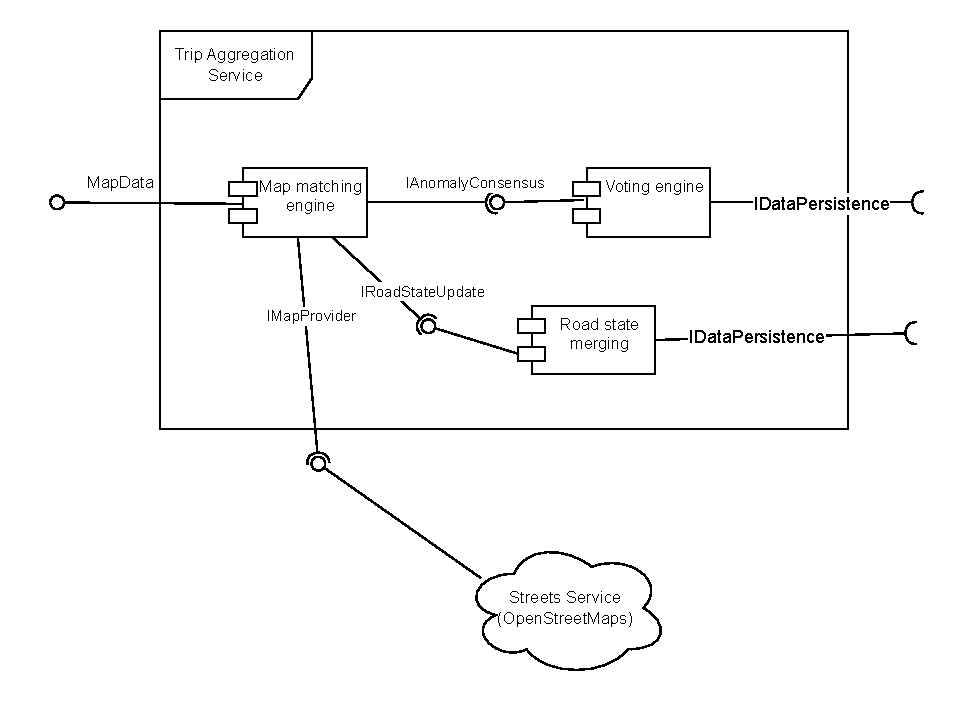
\includegraphics[width=0.85\textwidth]{Images/PDF/trip_aggr_arch.pdf}
      \caption{Trip Aggregation Service Internal Architecture}
      \label{fig:trip-aggregation-arch}
\end{figure}

\par The Trip Aggregation Service represents the core decision-making unit of the backend pipeline. To transform noisy telemetry streams into authoritative road data, it is internally decomposed into three specialized sub-components:

\begin{itemize}
      \item \textbf{Map Matching Engine}: This component acts as the entry point for validated trip data. It is responsible for aligning raw GPS coordinates to the actual road network topology. It interacts with the external \textit{Streets Service} (OpenStreetMap) to retrieve road segment metadata (Edge IDs), ensuring that spatial data from different users is correctly associated with the corresponding physical street segments.

      \item \textbf{Voting Engine}: This component implements the consensus logic for discrete anomalies. It receives map-matched anomaly reports (e.g., potential potholes) and applies a majority voting algorithm. An anomaly is confirmed as a verified obstacle only if it is reported by a significant number of distinct users within a specific time and space window, filtering out false positives.

      \item \textbf{Road State Merging}: This component processes continuous road metrics, such as average speed and surface roughness. It employs weighted moving average algorithms to merge new telemetry data with the historical state of the road segments stored in the database. This ensures that the global view of the road conditions evolves smoothly over time, mitigating the impact of outlier measurements.
\end{itemize}
\section{Deployment View}
\label{sec:deployment-view}%

\begin{figure}[H]
      \centering
      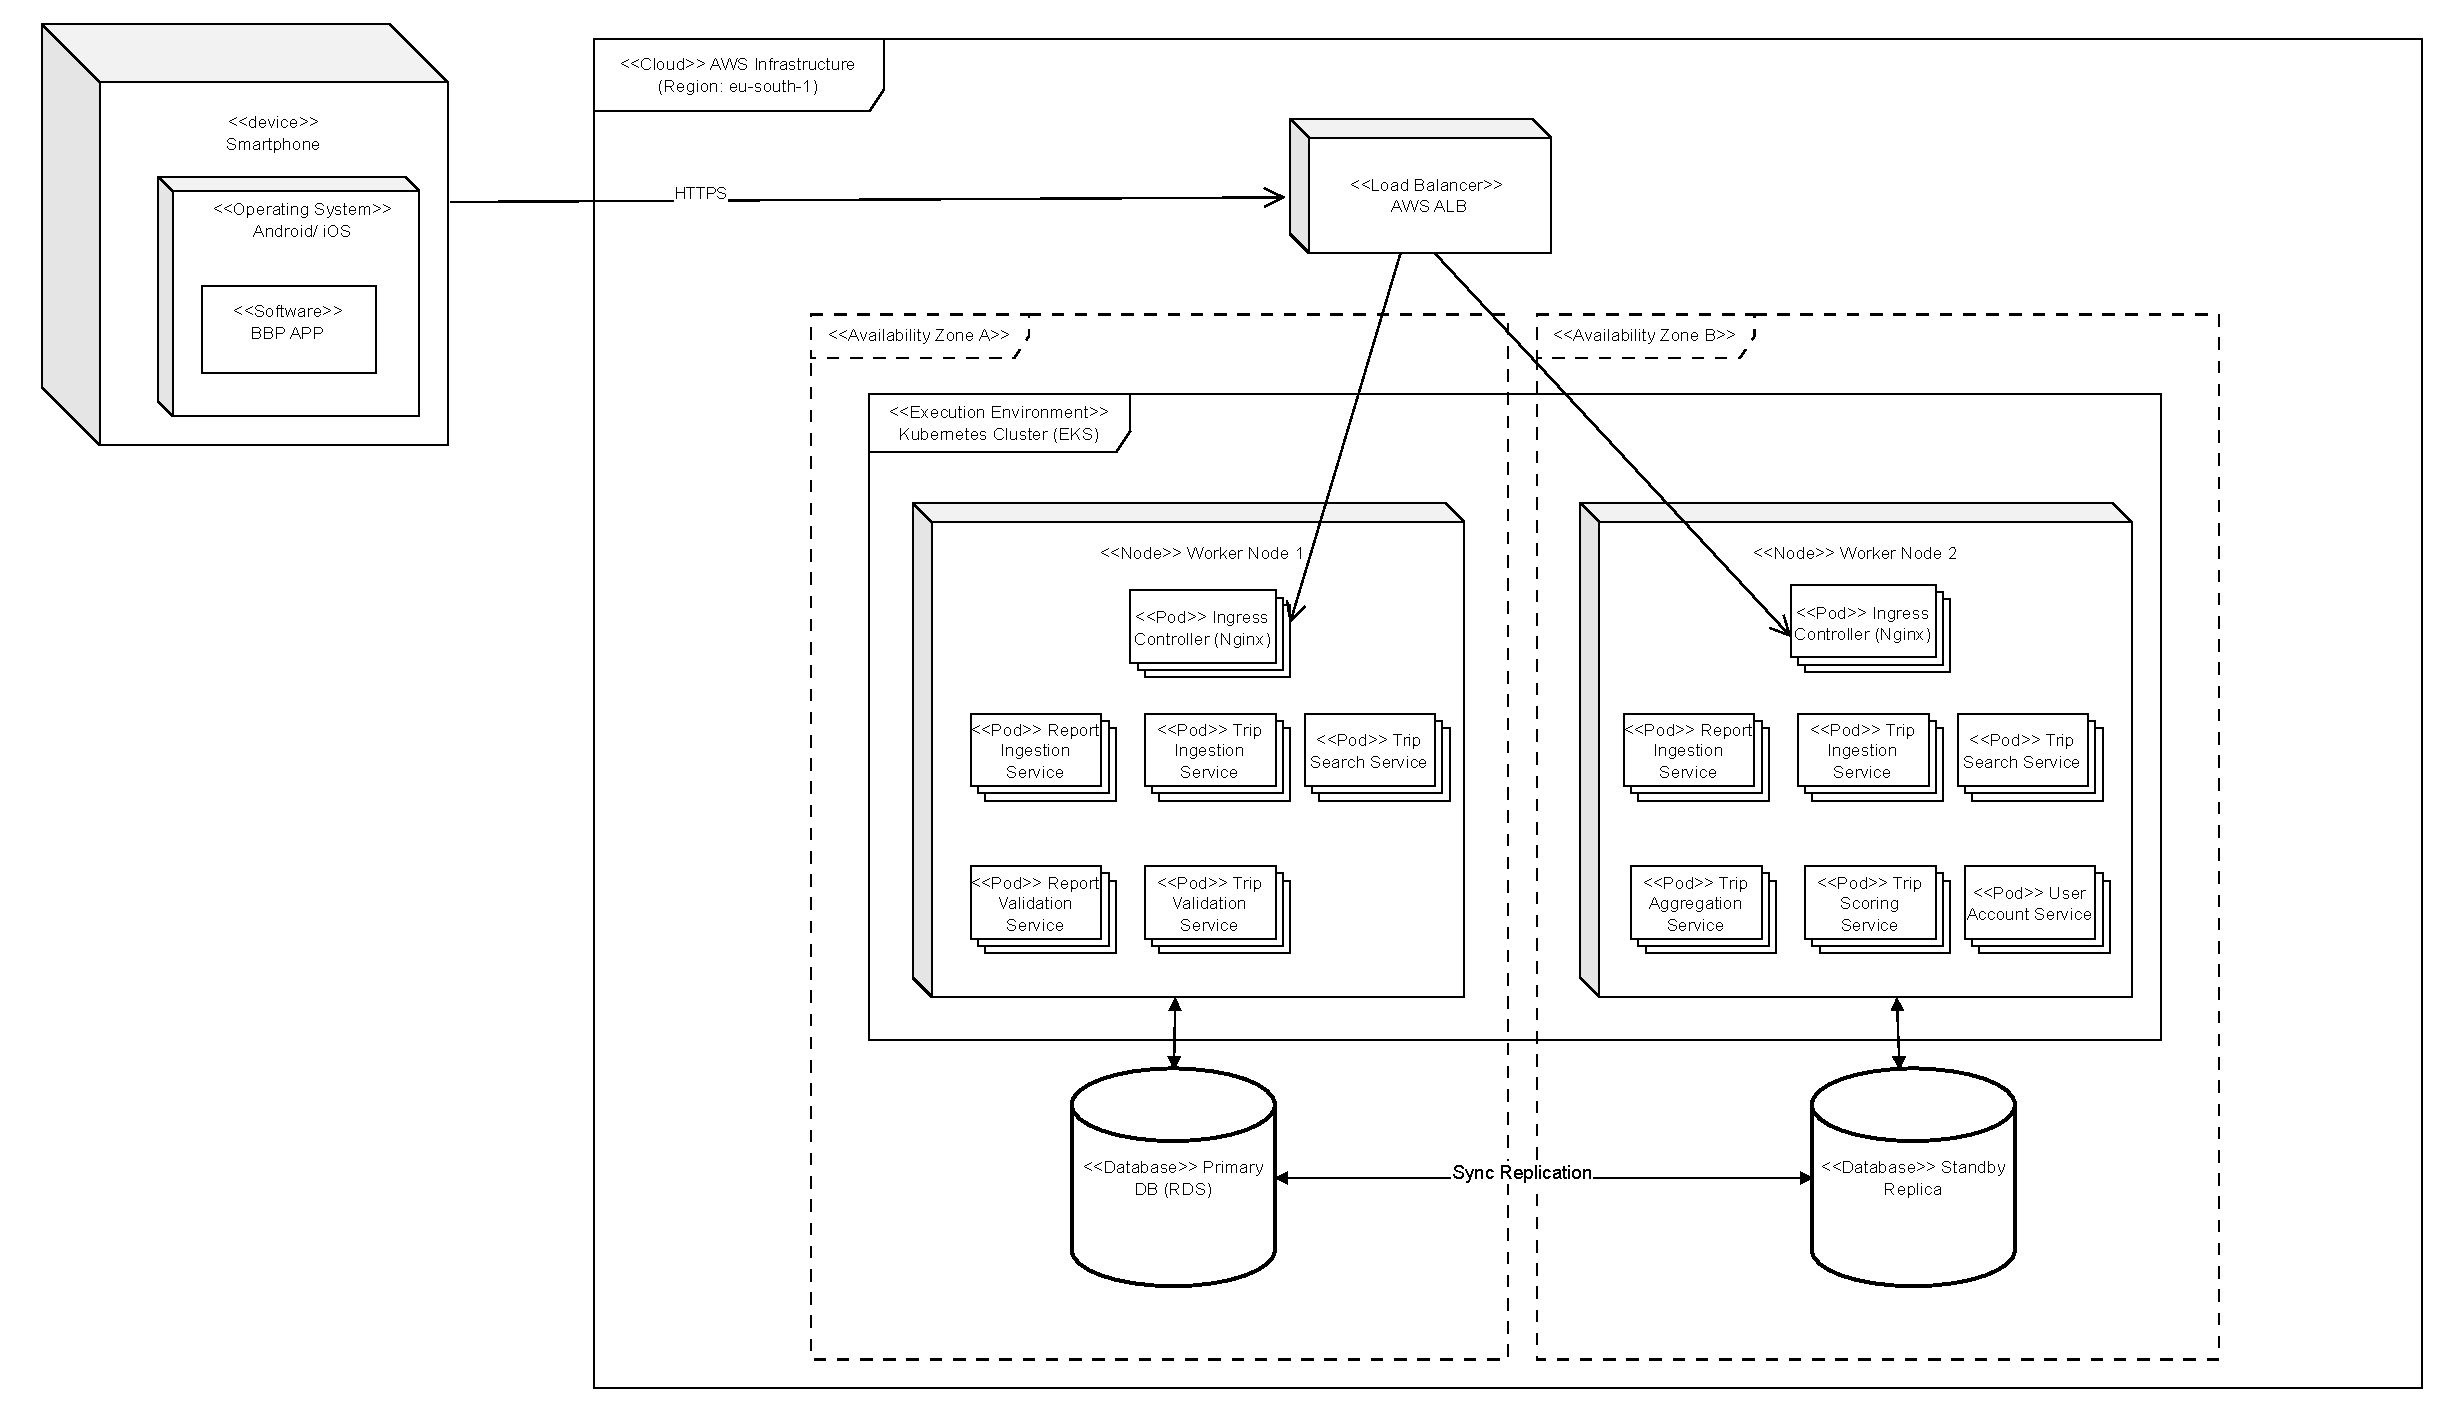
\includegraphics[width=0.85\textwidth]{Images/PDF/DeploymentView.pdf}
      \caption{Deployment Diagram}
      \label{fig:deployment-diagram}
\end{figure}

\subsubsection{Detailed Cluster Configuration}

Within the Kubernetes environment, specific resource objects are utilized to manage networking and configuration:

\begin{itemize}
    \item \textbf{Ingress Controller (Nginx):} Handles internal routing of HTTPS requests. It maps external URLs (e.g., \texttt{/api/trips}) to the appropriate internal services.
    \item \textbf{Kubernetes Services:} Provide stable internal IP addresses and DNS names (Service Discovery), allowing pods to communicate (e.g., \textit{Aggregation Service} calling \textit{Streets Service}) regardless of the ephemeral nature of individual pod instances.
    \item \textbf{Secrets \& ConfigMaps:} Decouple configuration from code. Database credentials and external API keys (e.g., OpenWeatherMap key) are stored as \textit{Secrets} and injected securely into the containers at runtime.
\end{itemize}

\subsubsection{Storage Technologies}
The architecture employs a \textbf{Polyglot Persistence} strategy tailored to the data nature:
\begin{itemize}
    \item \textbf{AWS RDS (PostgreSQL + PostGIS):} Used for structured business data (Users, Reports) and geospatial queries (finding obstacles within a radius).
    \item \textbf{AWS Timestream (or InfluxDB):} A specialized Time-Series database used to store the high-volume, append-only stream of raw sensor telemetry (accelerometer/GPS traces) for historical analysis.
\end{itemize}
\section{Runtime View}
\label{sec:runtime-view}%

% RV 01a
\subsection{Local Trip Recording and Monitoring}
\label{sub:local-trip-recording}

\begin{figure}[H]
      \centering
      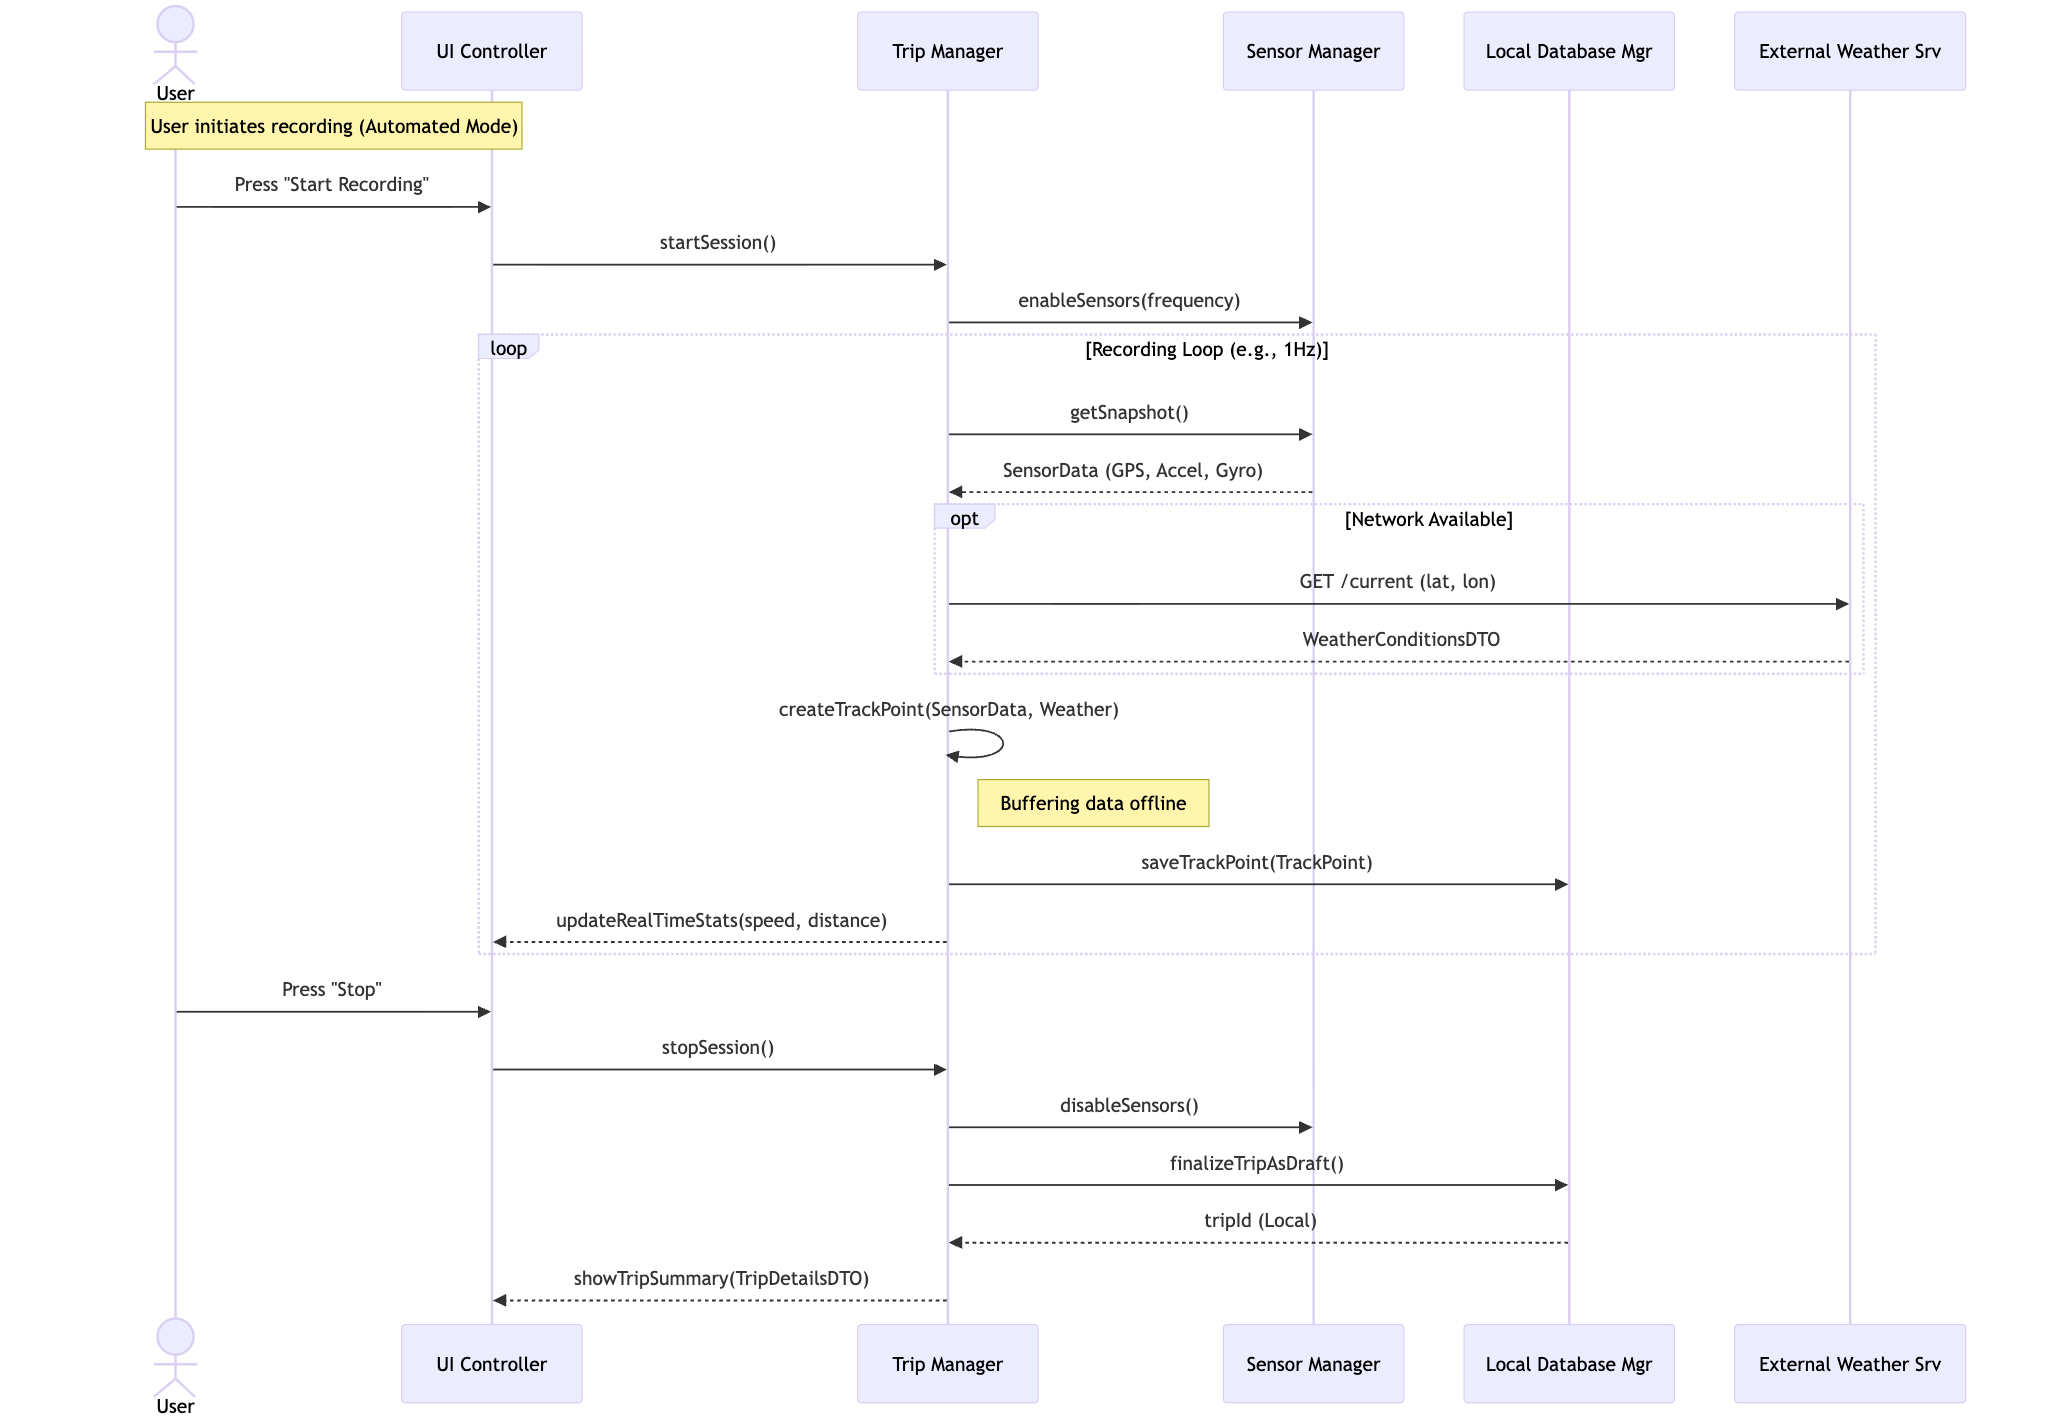
\includegraphics[width=0.95\textwidth]{Images/SEQ/aut_trip.png}
      \caption{Runtime View - Local Trip Recording}
      \label{fig:local_recording_sequence}
\end{figure}

\par Figure \ref{fig:local_recording_sequence} illustrates the data acquisition loop on the mobile device. This process is designed to ensure robust sensor data collection and real-time user feedback, while maintaining full functionality even in offline conditions.

\begin{itemize}
    \item \textbf{Initialization:} The process begins when the user triggers the "Start Recording" action. The \textit{UI Controller} invokes the \textit{Trip Manager}, which initializes a new session and activates the hardware sensors via the \textit{Sensor Manager}.
    
    \item \textbf{Acquisition Loop:} During the ride, the \textit{Trip Manager} periodically polls the \textit{Sensor Manager} to retrieve a snapshot of the telemetry data (GPS coordinates, accelerometer, gyroscope). These raw readings are encapsulated into a \texttt{TrackPoint} object. Optionally, if network connectivity is available, the system attempts to fetch real-time context from the \textit{Weather Service} to enrich the user display.
    
    \item \textbf{Local Buffering:} To guarantee data integrity (Constraint C05), each \texttt{TrackPoint} is immediately persisted to the internal storage via the \textit{Local Database Manager}. This ensures that no data is lost in the event of an application crash or battery failure.
    
    \item \textbf{Finalization:} When the user stops the recording, the \textit{Trip Manager} consolidates the buffered data into a \texttt{TripUploadDTO} structure (setting the status to DRAFT) and finalizes the record in the local database. The trip is now ready for review or deferred upload.
\end{itemize}
\subsection{Trip Upload and Synchronization}
\label{sub:trip-upload}

\begin{figure}[H]
      \centering
      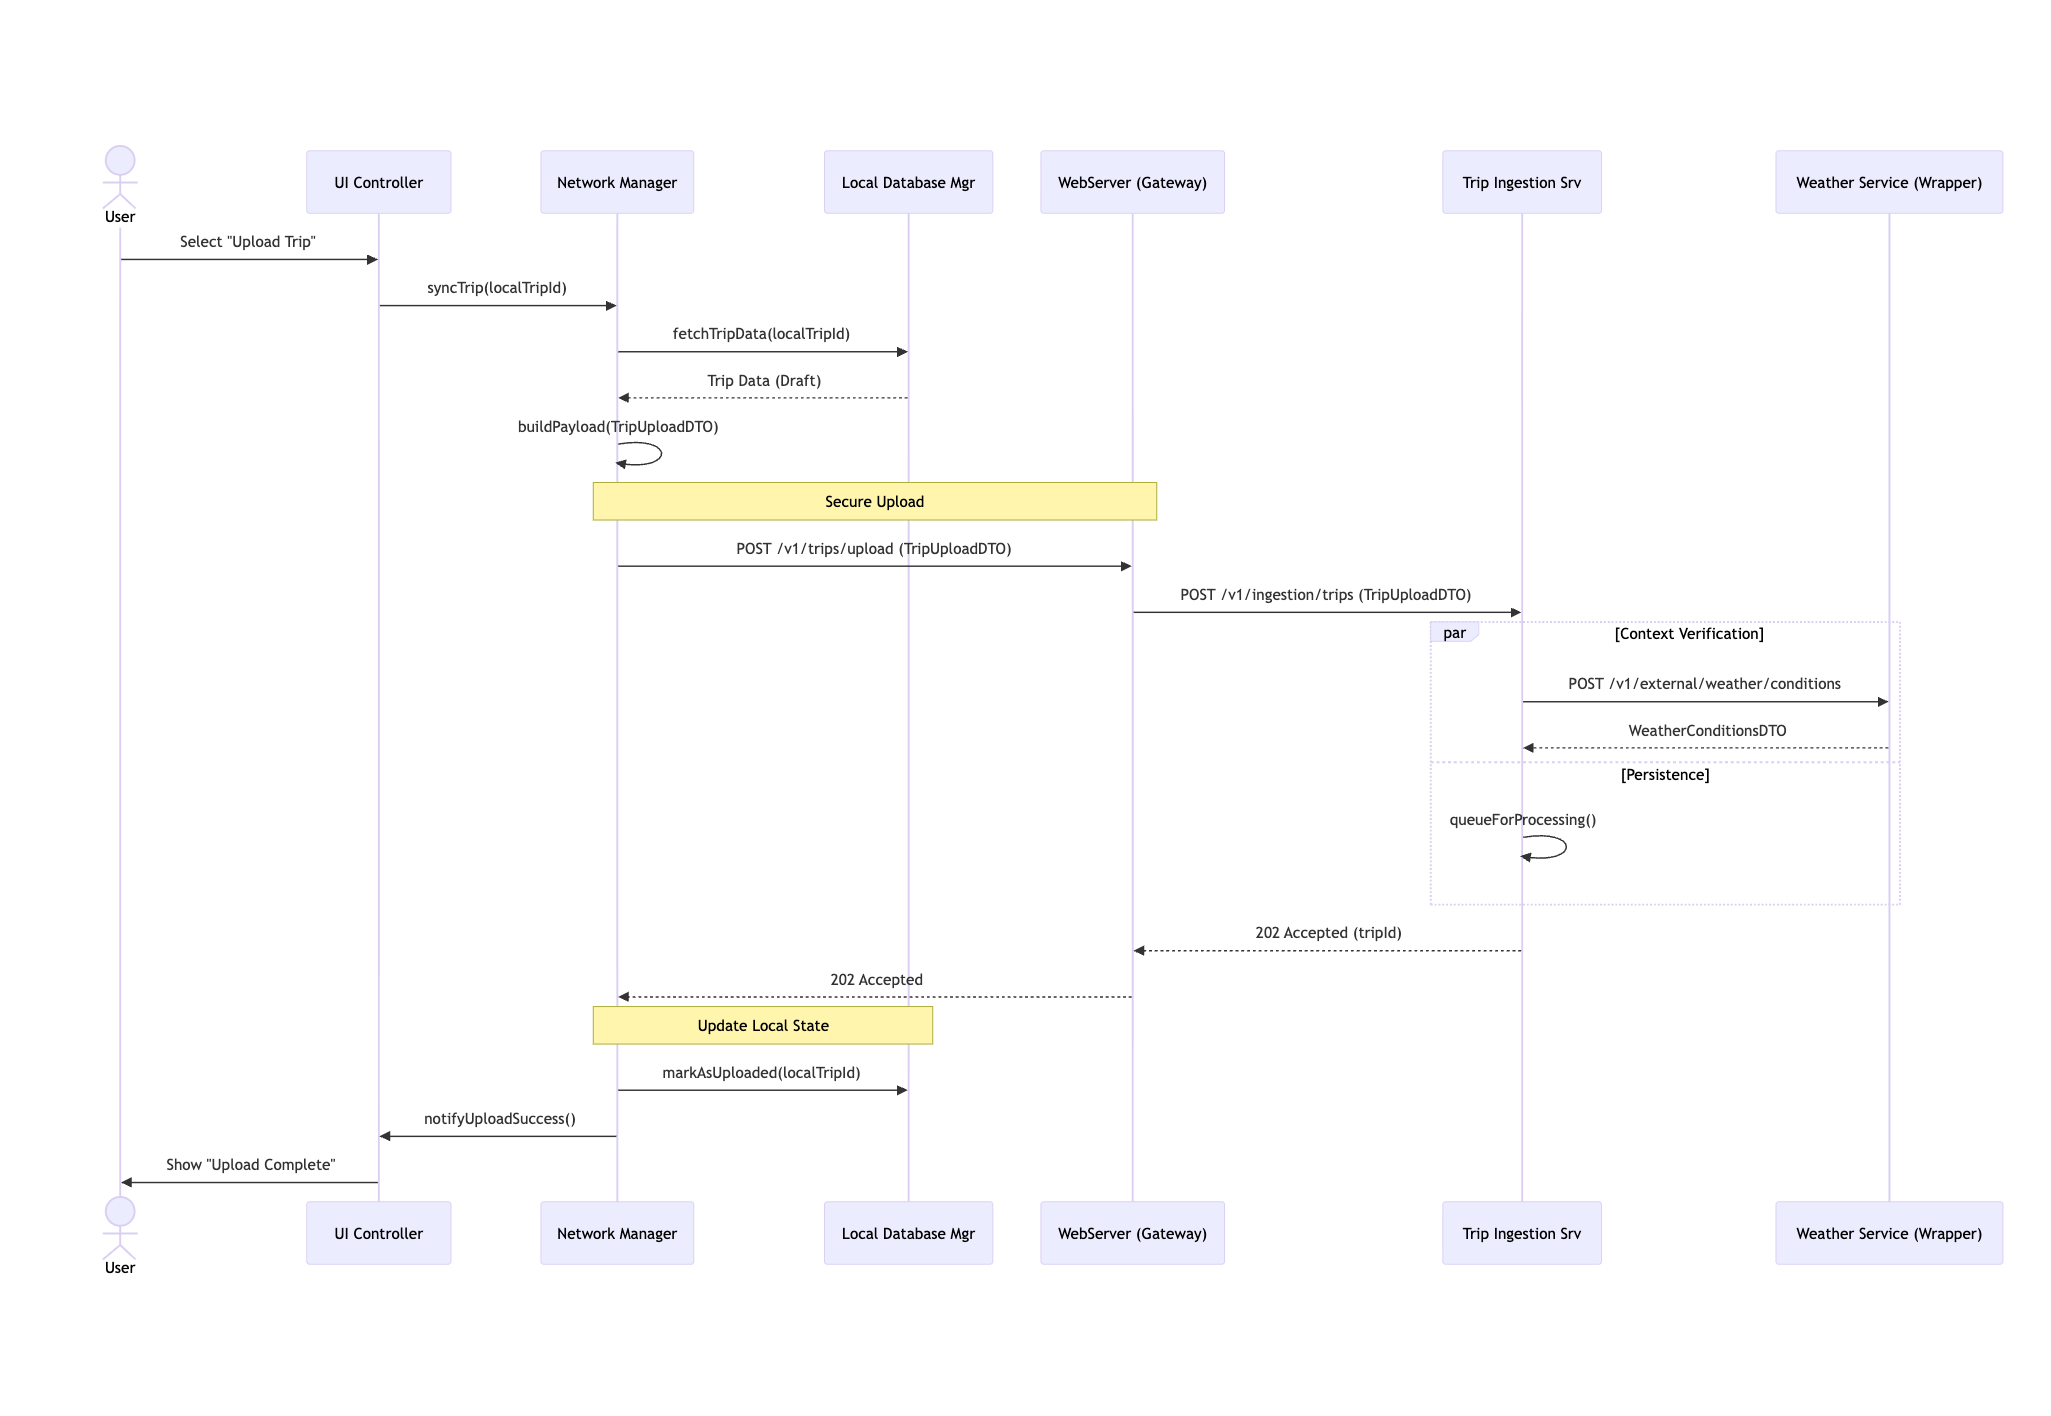
\includegraphics[width=0.95\textwidth]{Images/SEQ/upload_trip.png}
      \caption{Runtime View - Trip Upload and Synchronization}
      \label{fig:upload_sequence}
\end{figure}

\par Figure \ref{fig:upload_sequence} details the synchronization workflow. This phase ensures that locally stored trip data is securely transmitted to the backend for processing.

\begin{itemize}
    \item \textbf{Upload Initiation:} The process is triggered by the user (or automatically upon network recovery). The \textit{Network Manager} first interacts with the \textit{Local Database Manager} to retrieve the complete trip payload, encapsulated in a \texttt{TripUploadDTO}.
    
    \item \textbf{Data Ingestion:} The \textit{Network Manager} establishes a secure HTTPS connection with the \textit{WebServer} (API Gateway) and invokes the \texttt{POST /v1/trips/upload} endpoint. The Gateway routes this request to the internal \textit{Trip Ingestion Service} via \texttt{POST /v1/ingestion/trips}.
    
    \item \textbf{Verification and Queuing:} Upon receipt, the \textit{Trip Ingestion Service} performs a preliminary check by querying the \textit{Weather Service} (via \texttt{POST /v1/external/weather/conditions}) to validate the environmental metadata. It then persists the raw data in the \textit{Trips Data} store and places the task in a processing queue.
    
    \item \textbf{Asynchronous Acknowledgment:} To maximize responsiveness, the server immediately returns a \texttt{202 Accepted} status code once the data is safely queued. The \textit{Network Manager} receives this confirmation and instructs the \textit{Local Database Manager} to mark the trip as "Uploaded", finalizing the synchronization on the client side.
\end{itemize}% RV 02
\subsection{Backend Data Processing Pipeline}
\label{sub:backend-pipeline}

\begin{figure}[H]
      \centering
      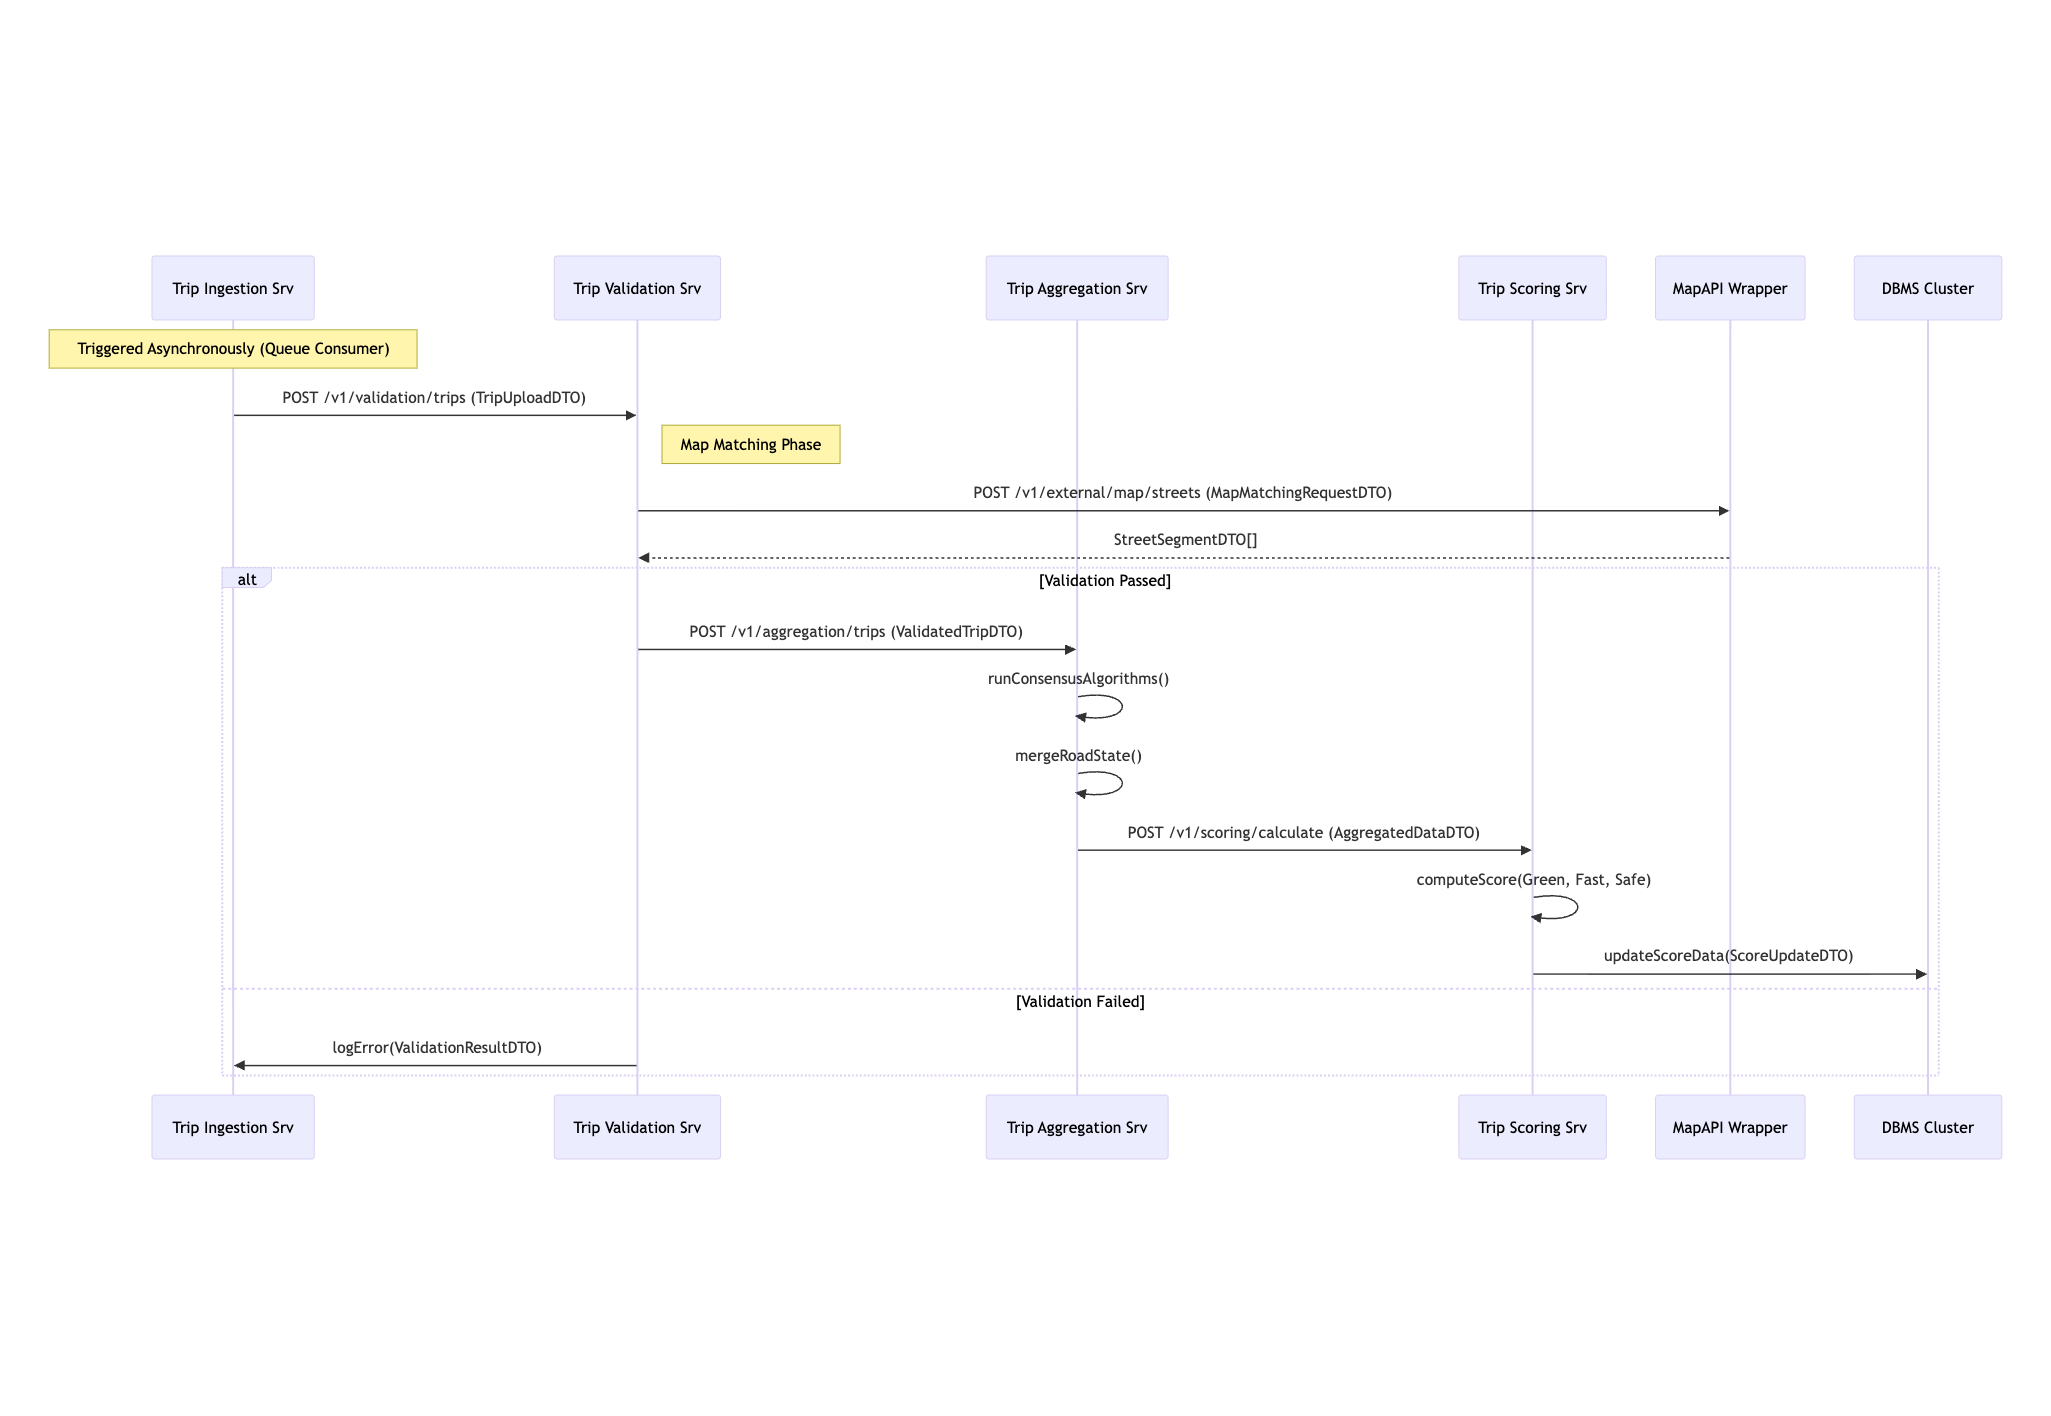
\includegraphics[width=0.95\textwidth]{Images/SEQ/backend_pipeline.png}
      \caption{Runtime View - Backend Data Processing Pipeline}
      \label{fig:pipeline_sequence}
\end{figure}

\par Figure \ref{fig:pipeline_sequence} illustrates the asynchronous processing workflow responsible for transforming raw telemetry into meaningful safety scores. This pipeline is triggered automatically by the \textit{Trip Ingestion Service} upon successful data persistence and focuses on the internal orchestration between microservices.

\begin{itemize}
    \item \textbf{Validation:} The process begins when the \textit{Trip Ingestion Service} dequeues the raw trip and invokes the \textit{Trip Validation Service} via \texttt{POST /v1/validation/trips}. This component verifies the data consistency and filters GPS noise. Crucially, it performs map-matching by querying the external \textit{Streets Service} (via \texttt{POST /v1/external/map/streets}) to ensure the recorded points correspond to valid road segments.
    
    \item \textbf{Aggregation:} Once validated, the data is forwarded to the \textit{Trip Aggregation Service} using the \texttt{ITripAggregation} interface. Here, the service merges the new trajectory with the historical state of the road segments. This involves running consensus algorithms (via the internal \textit{Voting Engine}) to confirm any reported anomalies.
    
    \item \textbf{Scoring:} The updated segment data is then sent to the \textit{Trip Scoring Service} via \texttt{POST /v1/scoring/calculate}. This engine recalculates the Quality of Experience (QoE) score for the affected paths based on the new averages (roughness, speed, safety).
    
    \item \textbf{Final Persistence:} Finally, the new scores are persisted in the \textit{Score Data} store via the \texttt{IDataPersistence} interface, making them immediately available for future search queries.
\end{itemize}
\subsection{Trip Search and Visualization}
\label{sub:trip-search}

\begin{figure}[H]
      \centering
      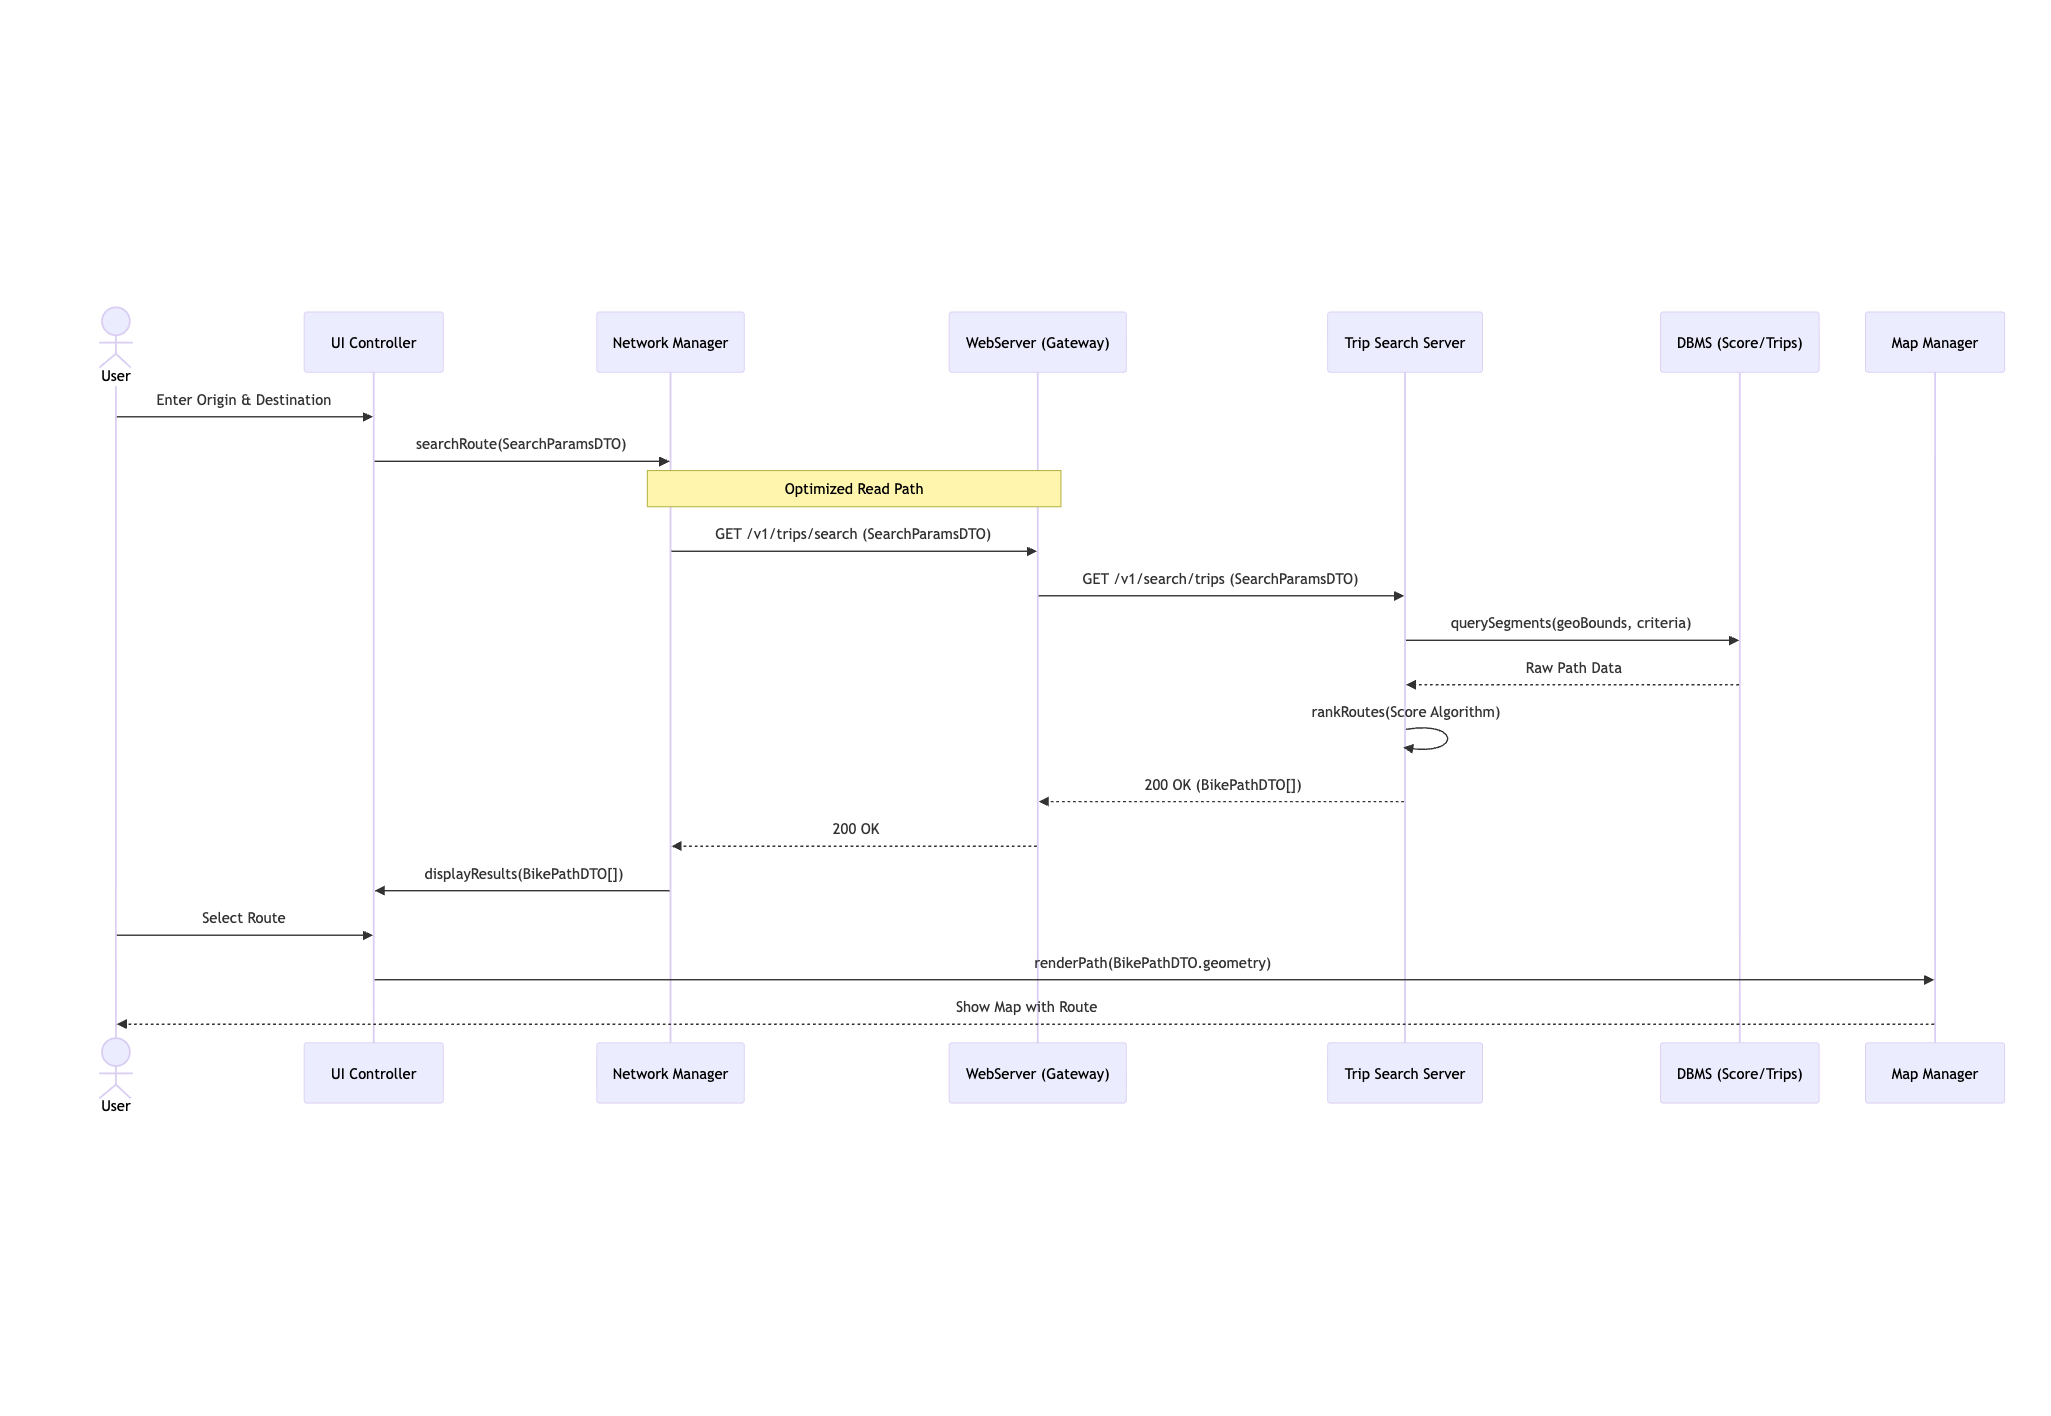
\includegraphics[width=0.95\textwidth]{Images/SEQ/search_path.png}
      \caption{Runtime View - Trip Search and Visualization}
      \label{fig:search_sequence}
\end{figure}

\par Figure \ref{fig:search_sequence} depicts the execution flow for the Route Search scenario. This workflow demonstrates the implementation of the \textit{Command Query Responsibility Segregation} (CQRS) pattern, where read operations are decoupled from the write pipeline.

\begin{itemize}
    \item \textbf{Search Initiation:} The user inputs the origin, destination, and preferences (e.g., "Safe Route") via the \textit{UI Controller}. The \textit{Network Manager} wraps these parameters into a \texttt{SearchParamsDTO} and sends a \texttt{GET /v1/trips/search} request to the \textit{WebServer}.
    
    \item \textbf{Dedicated Search Handling:} The \textit{WebServer} identifies the read-only nature of the request and routes it directly to the specialized \textit{Trip Search Server} via the \texttt{ITripQuery} interface (\texttt{GET /v1/search/trips}). This path avoids the computationally intensive ingestion components, ensuring responsiveness.
    
    \item \textbf{Data Retrieval and Ranking:} The \textit{Trip Search Server} executes optimized spatial queries against the \textit{Score Data} and \textit{Trips Data} stores to retrieve candidate segments. It then ranks the results based on their calculated QoE score and returns a list of \texttt{BikePathDTO} objects.
    
    \item \textbf{Visualization:} Upon receiving the results, the user selects a specific route. The \textit{UI Controller} invokes the \textit{Map Manager} to render the path geometry (contained in the DTO) on the interactive map, using color-coding to indicate the safety status of different segments.
\end{itemize}
\subsection{Manual Obstacle Reporting}
\label{sub:manual-reporting}

\begin{figure}[H]
      \centering
      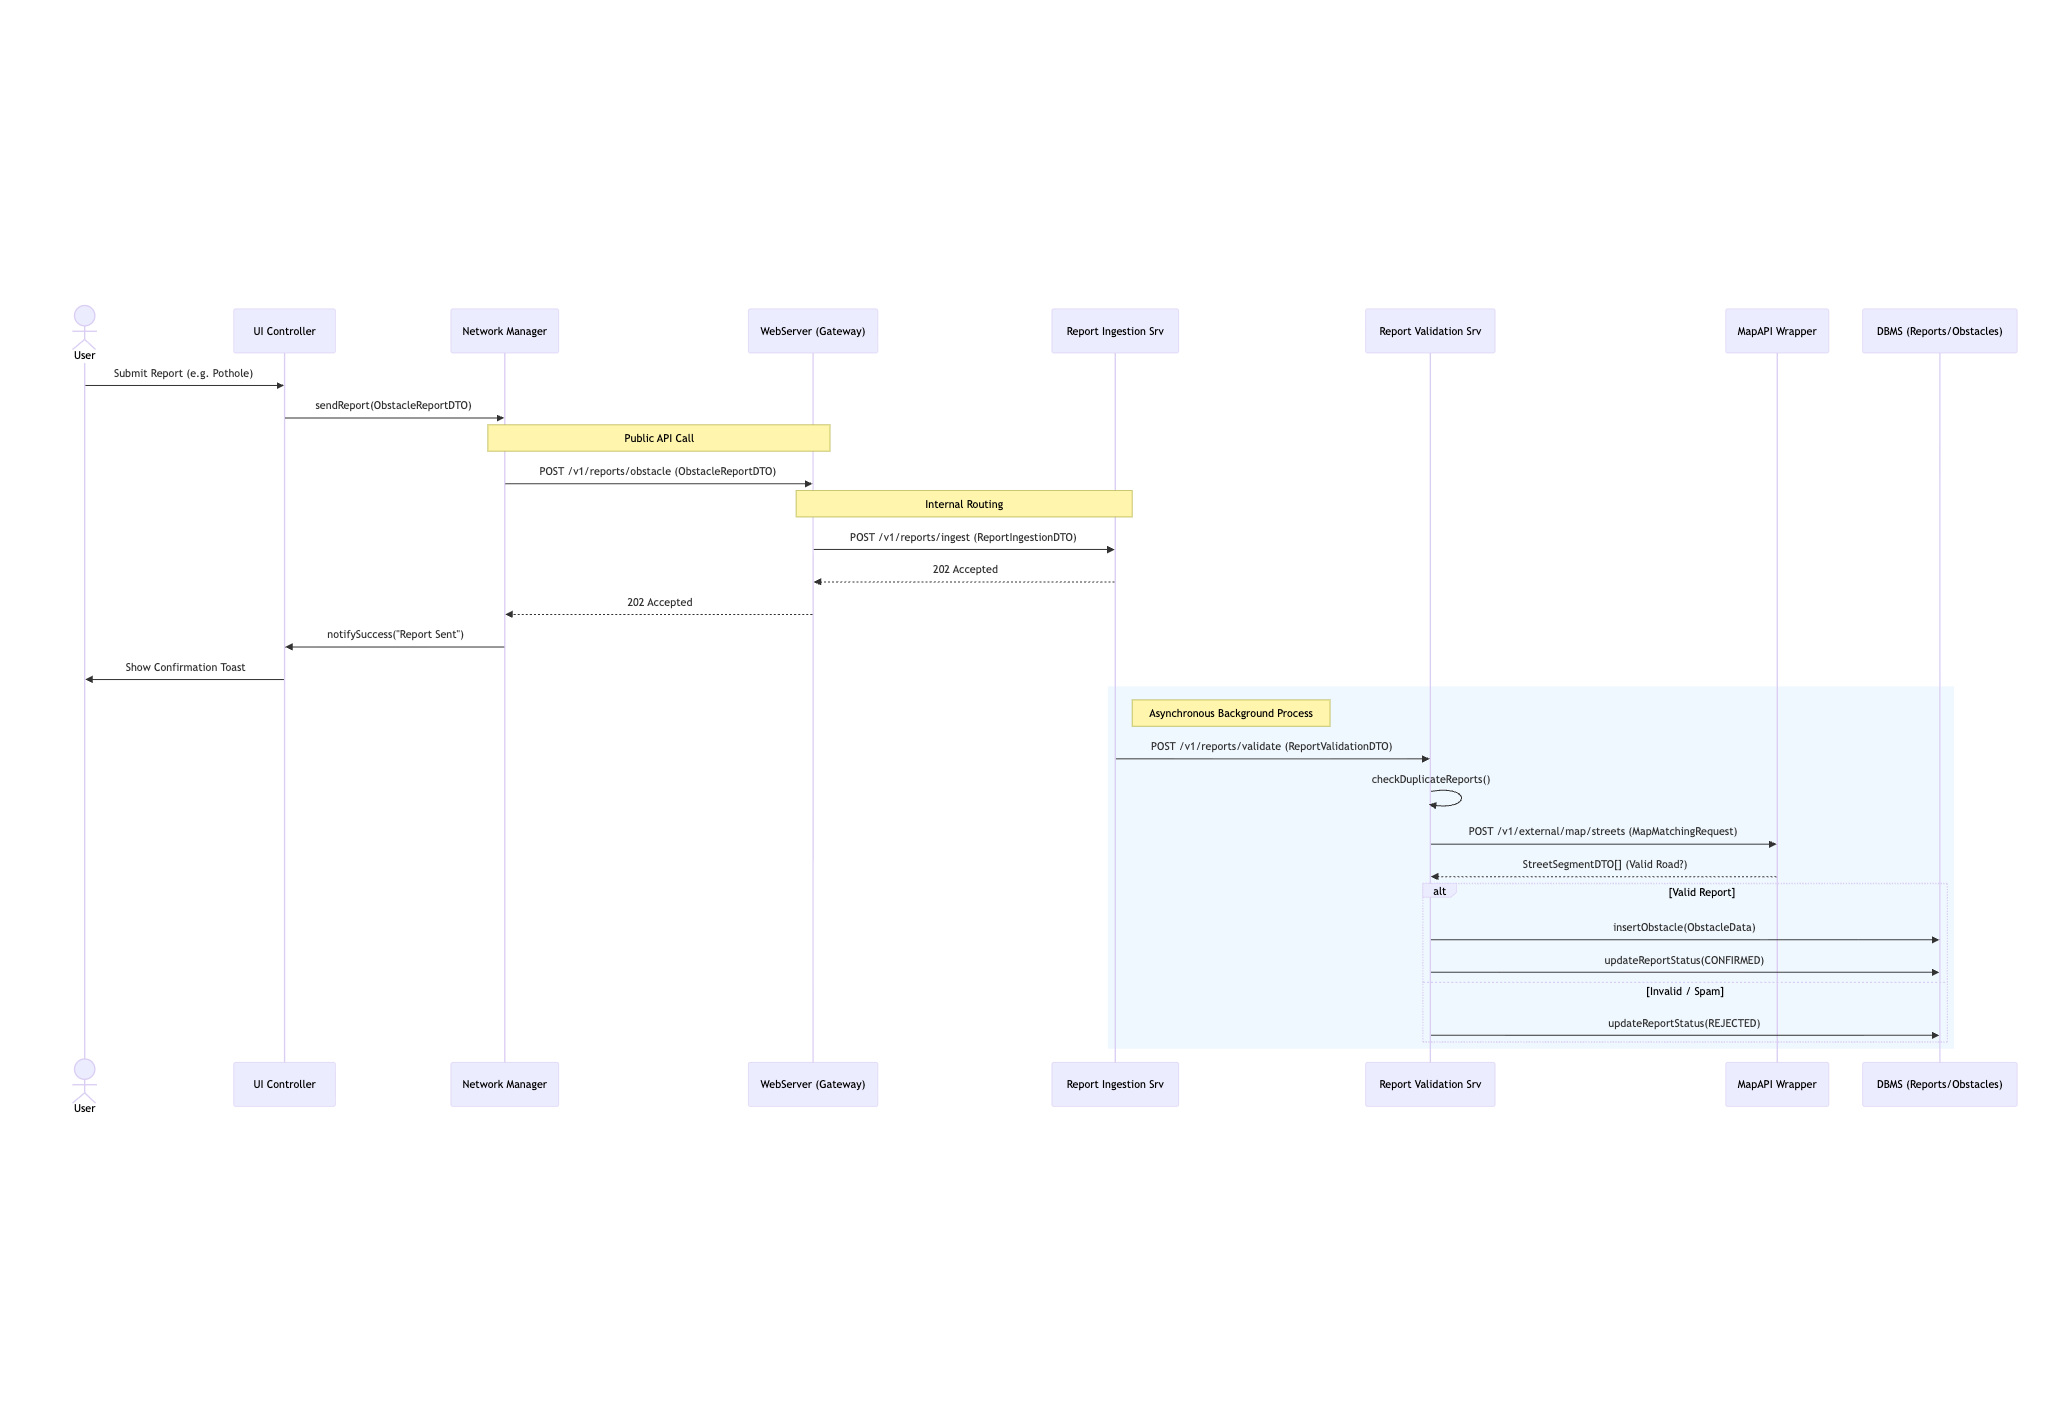
\includegraphics[width=0.95\textwidth]{Images/SEQ/report_submission.png}
      \caption{Runtime View - Manual Obstacle Reporting}
      \label{fig:reporting_sequence}
\end{figure}

\par Figure \ref{fig:reporting_sequence} details the interaction flow for the Manual Reporting scenario, where users contribute to the system by flagging road hazards (e.g., potholes). This process is managed by the dedicated \textit{Report Server} to ensure that crowd-sourced data ingestion does not impact the performance of real-time trip tracking.

\begin{itemize}
    \item \textbf{Submission:} The user fills out the report details (type, severity, description) via the \textit{UI Controller}. The \textit{Network Manager} wraps this information into an \texttt{ObstacleReportDTO} and transmits it to the \textit{WebServer} via a secure \texttt{POST /v1/reports/obstacle} request.
    
    \item \textbf{Ingestion and Acknowledgment:} The \textit{WebServer} forwards the request to the internal \textit{Report Ingestion Service} (mapping it to the \texttt{IReportManagement} interface). To maintain a responsive user experience, the service immediately queues the task and returns a \texttt{202 Accepted} status code. This allows the mobile app to confirm the action to the user without waiting for the validation process.
    
    \item \textbf{Asynchronous Validation:} In the background, the \textit{Report Ingestion Service} wraps the data into a \texttt{ReportValidationDTO} and triggers the \textit{Report Validation Service}. This component verifies the spatial consistency of the report by querying the external \textit{Streets Service} (Map Matching) to ensure the coordinates correspond to a valid road segment.
    
    \item \textbf{Persistence:} Upon successful validation, the service persists the confirmed obstacle in the \textit{Reports Data} store using the \texttt{IDataPersistence} interface, making the hazard visible to other cyclists in future searches.
\end{itemize}
\subsection{User Authentication}
\label{sub:user-auth}

\begin{figure}[H]
      \centering
      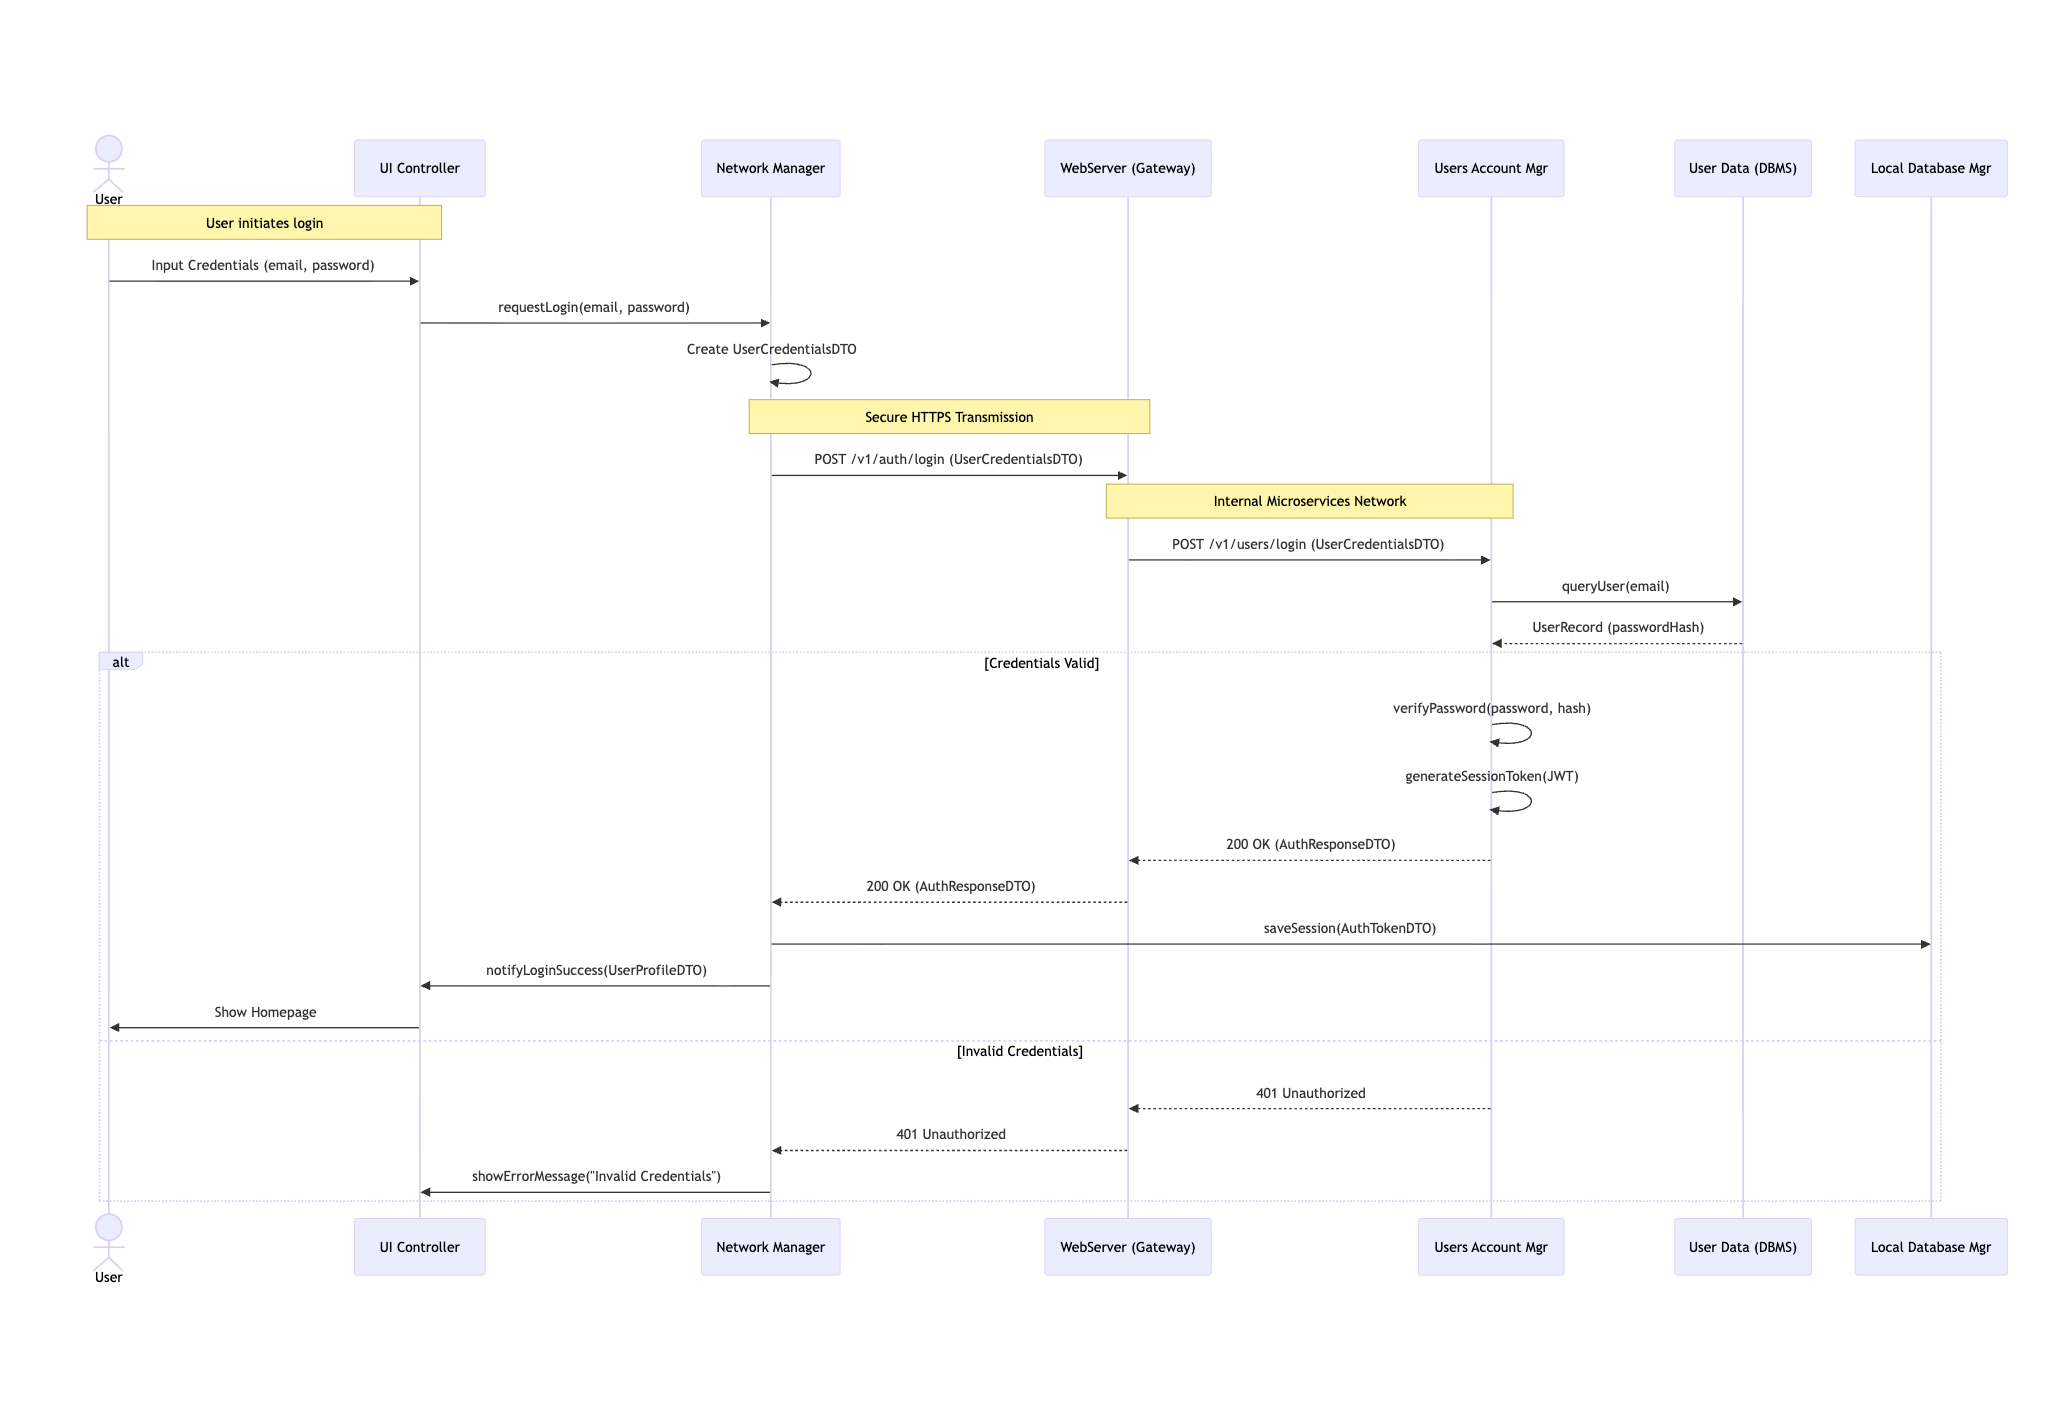
\includegraphics[width=0.95\textwidth]{Images/SEQ/login.png} %
      \caption{Runtime View - User Authentication}
      \label{fig:seq_auth}
\end{figure}
\par Figure \ref{fig:seq_auth} illustrates the authentication workflow for registered users. This process is managed by the specialized \textit{Users Account Manager Service} to ensure the secure handling of sensitive credentials, isolated from the trip processing logic.

\begin{itemize}
    \item \textbf{Credential Submission:} The user inputs their credentials via the \textit{UI Controller}. The \textit{Network Manager} wraps the inputs into a \texttt{UserCredentialsDTO} and transmits it to the \textit{WebServer} (API Gateway) via a secure HTTPS channel.

    \item \textbf{Authentication Logic:} The \textit{WebServer} delegates the verification request to the \textit{Users Account Manager Service} via the \texttt{IUserManagement} interface (specifically calling the \texttt{POST /users/login} endpoint). This component retrieves the stored user hash from the \textit{User Data} store and validates the provided password.

    \item \textbf{Session Management:} Upon successful verification, the service generates a secure authentication token (JWT) encapsulated in an \texttt{AuthResponseDTO}. The \textit{Mobile App} persists this token locally via the \textit{Local Database Manager} to maintain the session state for subsequent API calls (such as trip uploads or reporting).
\end{itemize}
\subsection{User Registration}
\begin{figure}[H]
      \centering
      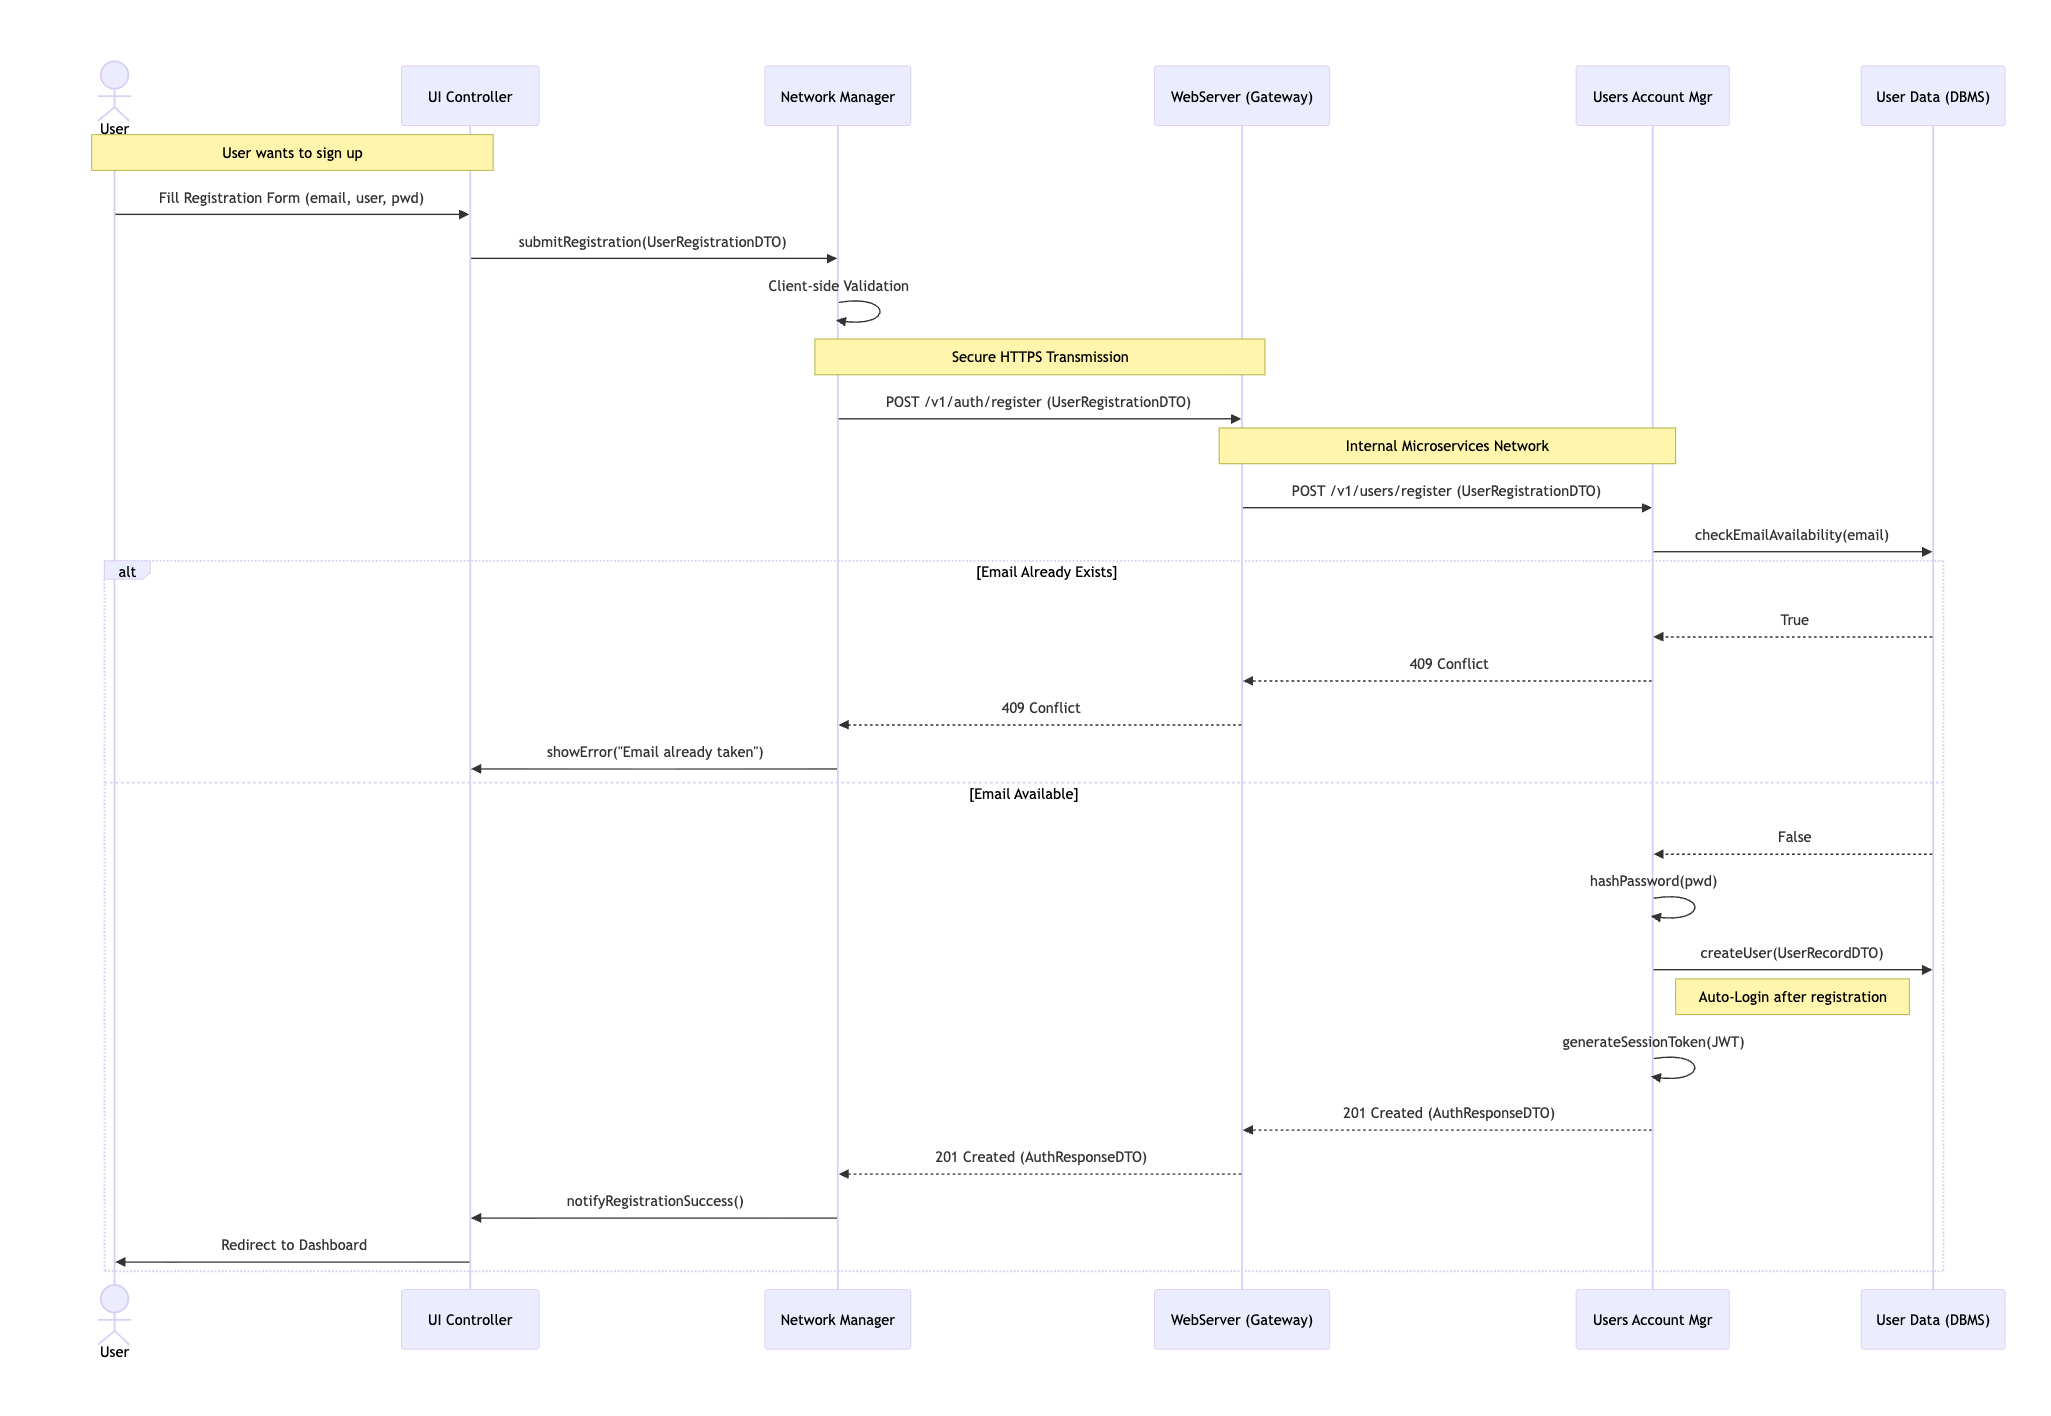
\includegraphics[width=0.95\textwidth]{Images/SEQ/signup.png} %
      \caption{Runtime View - User Registration}
      \label{fig:seq_auth}
\end{figure}
This scenario details the onboarding process for a new user. The workflow ensures data consistency by preventing duplicate accounts and securing user credentials before persistence.

\begin{itemize}
    \item \textbf{Data Submission}: The user submits their details via the \texttt{UI Controller}. The \texttt{Network Manager} validates the input format (e.g., email structure) and wraps the data into a \texttt{UserRegistrationDTO}.
    \item \textbf{Account Creation}: The API Gateway forwards the request to the \textit{Users Account Manager} (\texttt{POST /v1/users/register}). The service first queries the \textit{User Data} store to verify that the email address is unique.
    \item \textbf{Persistence and Auto-Login}: If the email is available, the service hashes the password and persists the new account. Upon success, it automatically generates an authentication token (JWT), returning an \texttt{AuthResponseDTO} (HTTP 201 Created) to allow immediate access without requiring a separate login step.
\end{itemize}
\subsection{Manual Trip Creation}
\label{sub:manual-trip-creation}

\begin{figure}[H]
      \centering
      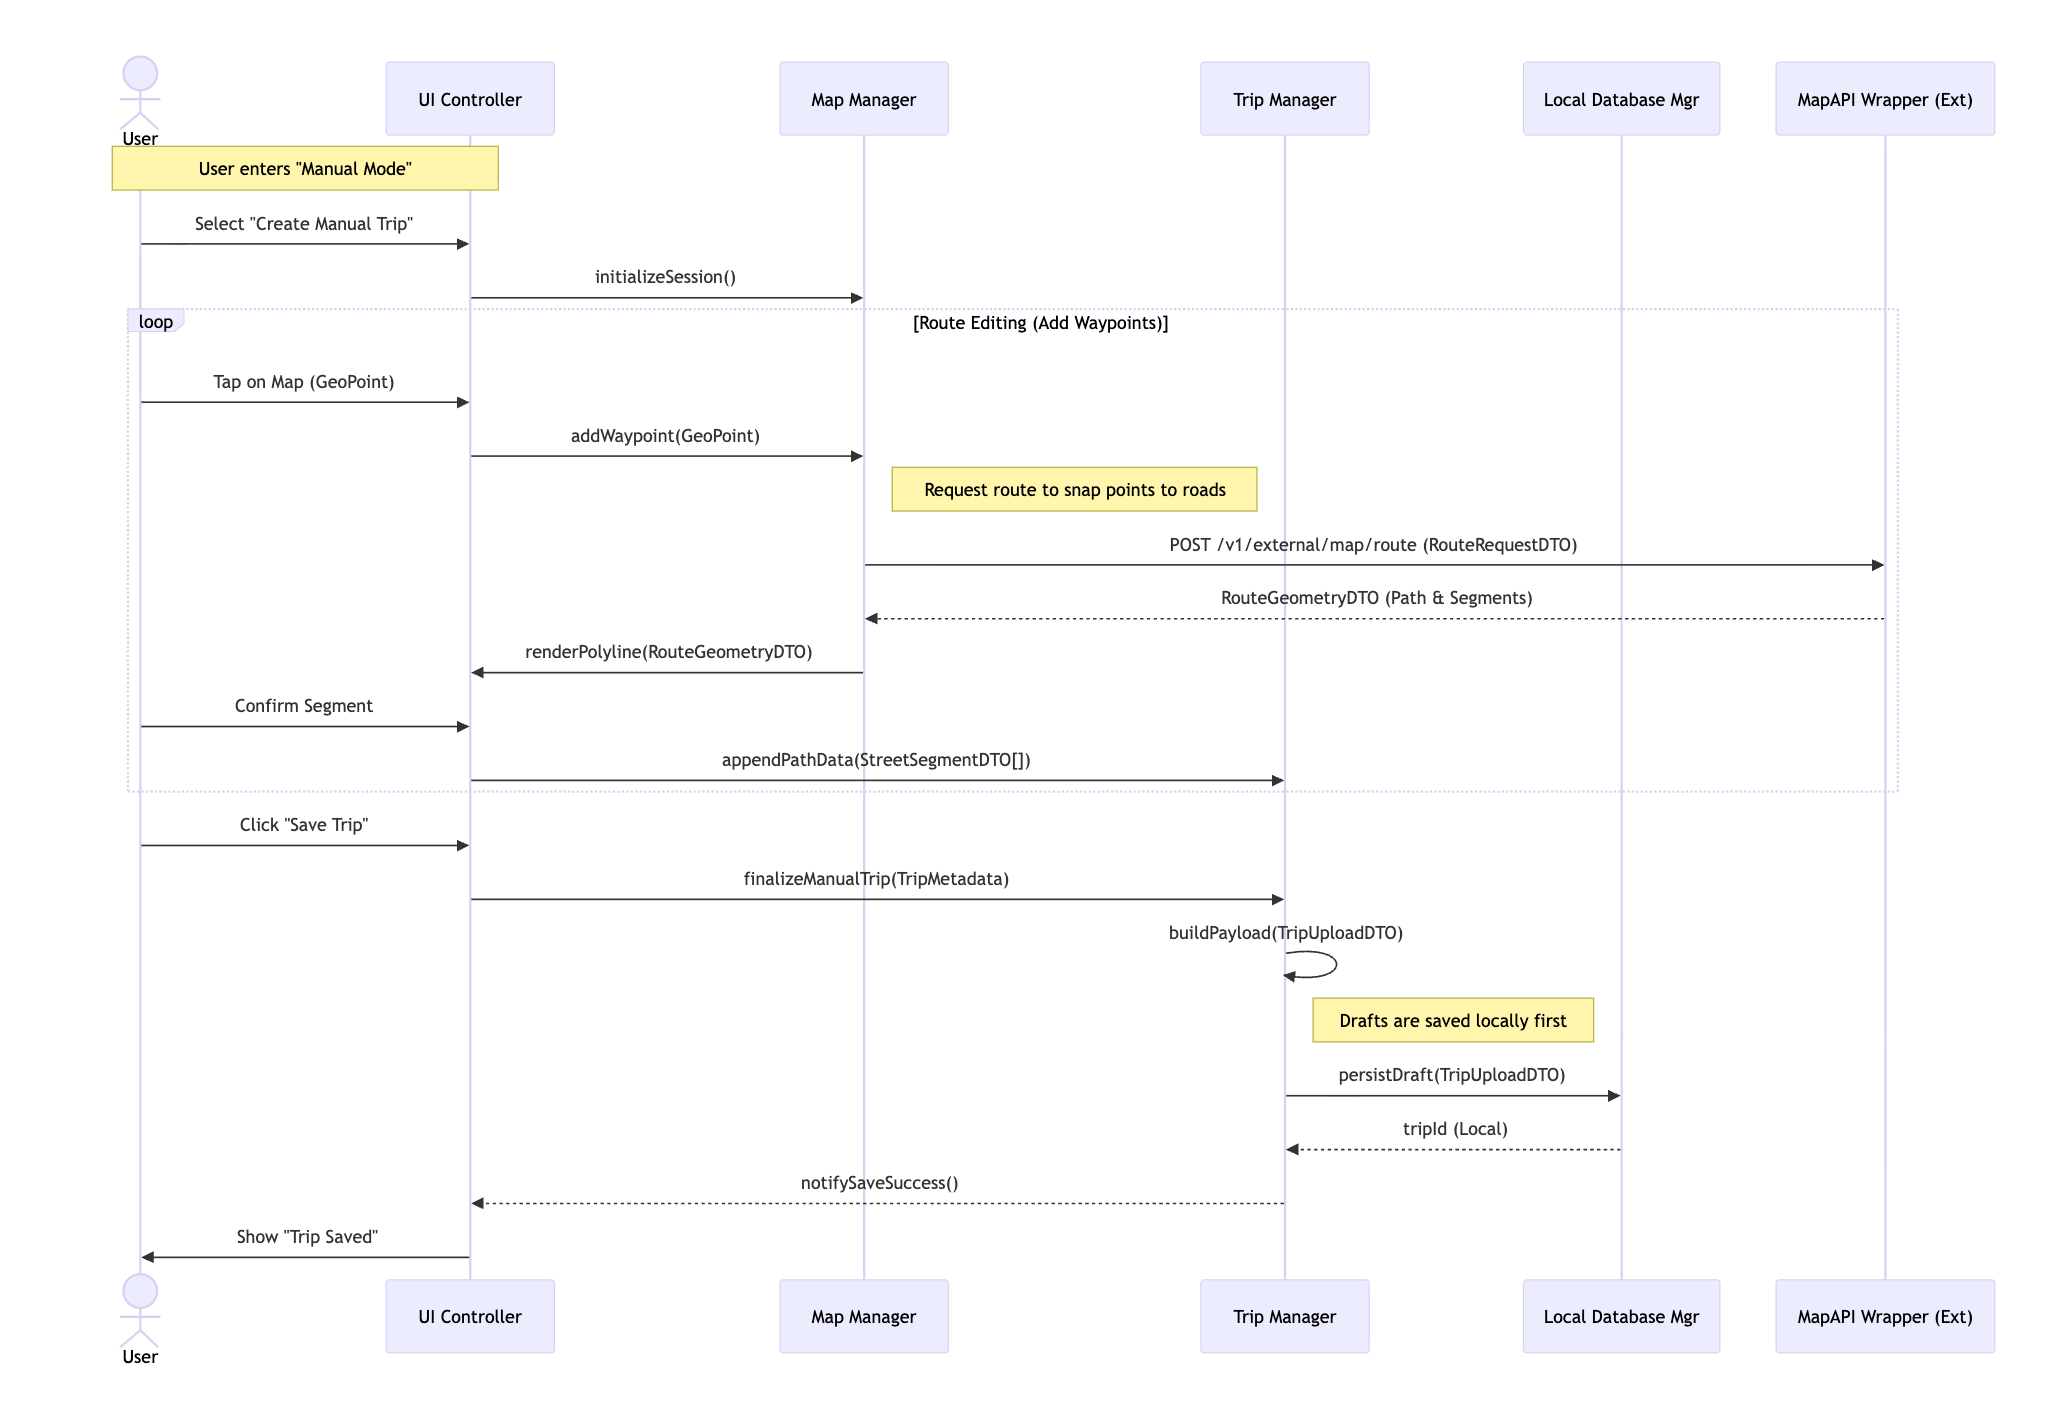
\includegraphics[width=0.95\textwidth]{Images/SEQ/manual_trip.png} % 
      \caption{Runtime View - Manual Trip Creation}
      \label{fig:manual_creation_sequence}
\end{figure}

\par Figure \ref{fig:manual_creation_sequence} illustrates the workflow for the \textit{Manual Trip Creation} scenario. This feature allows users to define a route and flag obstacles without physically traveling the path, relying on map interactions rather than sensor telemetry.

\begin{itemize}
    \item \textbf{Initialization:} The user enters the creation mode via the \textit{UI Controller}. The \textit{Map Manager} initializes a new session to handle user inputs on the map interface.
    
    \item \textbf{Map Interaction and Snapping:} The user interacts with the map to define waypoints (e.g., origin and destination). The \textit{Map Manager} captures these coordinates and invokes the external map provider via the \textit{MapAPI Wrapper} (specifically calling \texttt{POST /v1/external/map/route} with a \texttt{RouteRequestDTO}). This step "snaps" the raw points to the actual road network geometry, returning a precise \texttt{RouteGeometryDTO}.
    
    \item \textbf{Obstacle Injection:} The user can manually inject obstacle data (e.g., marking a known pothole on the drawn path). These inputs are captured by the \textit{Trip Manager} and associated with the corresponding road segment in the draft.
    
    \item \textbf{Persistence:} Once the route is confirmed, the \textit{Trip Manager} aggregates the segments into a \texttt{TripUploadDTO} (setting the \texttt{AcquisitionMode} to MANUAL) and persists it via the \textit{Local Database Manager}. The trip is saved as a local draft, ready to be uploaded using the standard synchronization pipeline described in Section \ref{sub:trip-upload}.
\end{itemize}
% RV 09
\section{Component Interfaces}
This section details the application programming interfaces (APIs) exposed by the system components. The data types referenced in the parameters (e.g., \texttt{PathStatus}, \texttt{GeoPoint}, \texttt{AcquisitionMode}) strictly adhere to the Domain Model defined in the RASD.

Where multiple attributes need to be transferred simultaneously, we define Data Transfer Objects (DTOs) to encapsulate the payload.

\subsubsection{Backend Services Interfaces}
The following interfaces define the interaction points for the server-side microservices.

\paragraph{Interface: IBBPClientAPI}
This interface is exposed to mobile and web clients via the API Gateway.
\begin{itemize}
    \item \textbf{POST} \texttt{/v1/auth/register}
    \begin{itemize}
        \item \textbf{Description:} Registers a new user account in the system.
        \item \textbf{Request DTO:} \texttt{UserRegistrationDTO} (email, username, password).
        \item \textbf{Response:} \texttt{UserProfileDTO} and authentication token upon success.
        \item \textbf{Client:} Mobile App (Network Manager)
        \item \textbf{Server:} Users Account Manager Service
    \end{itemize}
    
    \item \textbf{POST} \texttt{/v1/auth/login}
    \begin{itemize}
        \item \textbf{Description:} Authenticates a user and initiates a session.
        \item \textbf{Request DTO:} \texttt{UserCredentialsDTO} (email, password).
        \item \textbf{Response:} \texttt{AuthResponseDTO} containing a JWT token and \texttt{UserProfileDTO}.
        \item \textbf{Client:} Mobile App (Network Manager)
        \item \textbf{Server:} Users Account Manager Service
    \end{itemize}
    
    \item \textbf{POST} \texttt{/v1/trips/upload}
    \begin{itemize}
        \item \textbf{Description:} Uploads a complete trip (manual or automatic) for ingestion and processing.
        \item \textbf{Request DTO:} \texttt{TripUploadDTO} (containing \texttt{Trip} data, \texttt{TrackPoint[]}, optional \texttt{WeatherConditions}).
        \item \textbf{Response:} \texttt{202 Accepted} with a \texttt{tripId} for asynchronous processing.
        \item \textbf{Client:} Mobile App (Network Manager)
        \item \textbf{Server:} Trip Ingestion Service
    \end{itemize}
    
    \item \textbf{PUT} \texttt{/v1/trips/\{tripId\}/publish}
    \begin{itemize}
        \item \textbf{Description:} Publishes a previously saved draft trip, making it public and triggering aggregation.
        \item \textbf{Request DTO:} \texttt{TripPublishDTO} (e.g., desired public name).
        \item \textbf{Response:} \texttt{200 OK} with publication status.
        \item \textbf{Client:} Mobile App (Network Manager)
        \item \textbf{Server:} Trip Aggregation Service
    \end{itemize}
    
    \item \textbf{GET} \texttt{/v1/trips/search}
    \begin{itemize}
        \item \textbf{Description:} Searches for public bike paths based on geographic criteria and filters.
        \item \textbf{Query Params:} \texttt{SearchParamsDTO} (origin, destination, minScore, etc.).
        \item \textbf{Response:} \texttt{BikePathDTO[]} with summary information.
        \item \textbf{Client:} Mobile App or Web Client (Network Manager/UI Controller)
        \item \textbf{Server:} Trip Search Server
    \end{itemize}
    
    \item \textbf{GET} \texttt{/v1/trips/\{tripId\}}
    \begin{itemize}
        \item \textbf{Description:} Retrieves detailed information for a specific trip (private for owners, public for published trips).
        \item \textbf{Response:} \texttt{TripDetailsDTO} (full trip data, path, obstacles, weather).
        \item \textbf{Client:} Mobile App (Network Manager)
        \item \textbf{Server:} Trip Search Server
    \end{itemize}
    
    \item \textbf{POST} \texttt{/v1/reports/obstacle}
    \begin{itemize}
        \item \textbf{Description:} Submits a manual obstacle report from a user.
        \item \textbf{Request DTO:} \texttt{ObstacleReportDTO} (location, description, type, optional image).
        \item \textbf{Response:} \texttt{202 Accepted} with a \texttt{reportId}.
        \item \textbf{Client:} Mobile App (Network Manager)
        \item \textbf{Server:} Report Ingestion Service
    \end{itemize}
    
    \item \textbf{POST} \texttt{/v1/reports/path-status}
    \begin{itemize}
        \item \textbf{Description:} Submits a manual rating/status report for a specific bike path.
        \item \textbf{Request DTO:} \texttt{PathStatusReportDTO} (pathId, status, comment).
        \item \textbf{Response:} \texttt{202 Accepted}.
        \item \textbf{Client:} Mobile App (Network Manager)
        \item \textbf{Server:} Report Ingestion Service
    \end{itemize}
    
    \item \textbf{PUT} \texttt{/v1/profile}
    \begin{itemize}
        \item \textbf{Description:} Updates the profile of the authenticated user.
        \item \textbf{Request DTO:} \texttt{UserProfileUpdateDTO} (non-sensitive user information).
        \item \textbf{Response:} Updated \texttt{UserProfileDTO}.
        \item \textbf{Client:} Mobile App (Network Manager)
        \item \textbf{Server:} Users Account Manager Service
    \end{itemize}
\end{itemize}

\paragraph{Interface: ITripOperations (Used by Trip Ingestion Service)}
\begin{itemize}
    \item \textbf{POST} \texttt{/v1/ingestion/trips}
    \begin{itemize}
        \item \textbf{Description:} Internal endpoint for receiving raw trip data. Performs initial validation and triggers the processing pipeline.
        \item \textbf{Request DTO:} \texttt{TripUploadDTO}.
        \item \textbf{Response:} \texttt{202 Accepted}.
        \item \textbf{Client:} WebServer (API Gateway)
        \item \textbf{Server:} Trip Ingestion Service
    \end{itemize}
\end{itemize}

\paragraph{Interface: ITripCompliance (Used by Trip Validation Service)}
\begin{itemize}
    \item \textbf{POST} \texttt{/v1/validation/trips}
    \begin{itemize}
        \item \textbf{Description:} Validates trip data for consistency, filters GPS noise, and performs map-matching.
        \item \textbf{Request DTO:} \texttt{TripUploadDTO}.
        \item \textbf{Response:} \texttt{ValidatedTripDTO} or a list of validation errors.
        \item \textbf{Client:} Trip Ingestion Service
        \item \textbf{Server:} Trip Validation Service
    \end{itemize}
\end{itemize}

\paragraph{Interface: ITripAggregation (Used by Trip Aggregation Service)}
\begin{itemize}
    \item \textbf{POST} \texttt{/v1/aggregation/trips}
    \begin{itemize}
        \item \textbf{Description:} Merges validated trip data with the historical road state and runs consensus algorithms.
        \item \textbf{Request DTO:} \texttt{ValidatedTripDTO}.
        \item \textbf{Response:} \texttt{AggregationResultDTO} (summary of applied updates).
        \item \textbf{Client:} Trip Validation Service
        \item \textbf{Server:} Trip Aggregation Service
    \end{itemize}
\end{itemize}

\paragraph{Interface: IScoringCalculation (Used by Trip Scoring Service)}
\begin{itemize}
    \item \textbf{POST} \texttt{/v1/scoring/calculate}
    \begin{itemize}
        \item \textbf{Description:} Calculates or updates the quality and safety score for affected road segments.
        \item \textbf{Request DTO:} \texttt{AggregatedDataDTO} (from aggregation service).
        \item \textbf{Response:} \texttt{ScoreUpdateDTO} (new scores for paths).
        \item \textbf{Client:} Trip Aggregation Service
        \item \textbf{Server:} Trip Scoring Service
    \end{itemize}
\end{itemize}

\paragraph{Interface: IReportManagement (Used by Report Server)}
\begin{itemize}
    \item \textbf{POST} \texttt{/v1/reports/ingest}
    \begin{itemize}
        \item \textbf{Description:} Internal endpoint for ingesting user-generated reports.
        \item \textbf{Request DTO:} \texttt{ReportIngestionDTO} (wraps \texttt{ObstacleReportDTO} or \texttt{PathStatusReportDTO}).
        \item \textbf{Response:} \texttt{202 Accepted}.
        \item \textbf{Client:} WebServer (API Gateway)
        \item \textbf{Server:} Report Ingestion Service
    \end{itemize}
    
    \item \textbf{POST} \texttt{/v1/reports/validate}
    \begin{itemize}
        \item \textbf{Description:} Validates an ingested report (spatial consistency, duplicates) and updates its state.
        \item \textbf{Request DTO:} \texttt{ReportValidationDTO}.
        \item \textbf{Response:} \texttt{ValidationResultDTO}.
        \item \textbf{Client:} Report Ingestion Service
        \item \textbf{Server:} Report Validation Service
    \end{itemize}
\end{itemize}

\paragraph{Interface: ITripQuery (Used by Trip Search Server)}
\begin{itemize}
    \item \textbf{GET} \texttt{/v1/search/trips}
    \begin{itemize}
        \item \textbf{Description:} Executes complex read-only queries for bike paths. Optimized for low latency.
        \item \textbf{Query Params:} \texttt{SearchParamsDTO}.
        \item \textbf{Response:} \texttt{BikePathDTO[]}.
        \item \textbf{Client:} WebServer (API Gateway)
        \item \textbf{Server:} Trip Search Server
    \end{itemize}
\end{itemize}

\paragraph{Interface: IUserManagement (Used by Users Account Manager Service)}
\begin{itemize}
    \item \textbf{POST} \texttt{/v1/users/register}
    \begin{itemize}
        \item \textbf{Description:} Internal endpoint for creating a new user account.
        \item \textbf{Request DTO:} \texttt{UserRegistrationDTO}.
        \item \textbf{Response:} \texttt{UserRecordDTO} (internal user representation).
        \item \textbf{Client:} WebServer (API Gateway)
        \item \textbf{Server:} Users Account Manager Service
    \end{itemize}
    
    \item \textbf{POST} \texttt{/v1/users/login}
    \begin{itemize}
        \item \textbf{Description:} Internal endpoint for authenticating a user.
        \item \textbf{Request DTO:} \texttt{UserCredentialsDTO}.
        \item \textbf{Response:} \texttt{AuthTokenDTO} (JWT) and \texttt{UserRecordDTO}.
        \item \textbf{Client:} WebServer (API Gateway)
        \item \textbf{Server:} Users Account Manager Service
    \end{itemize}
\end{itemize}

\subsubsection{External Wrappers Interfaces}
These interfaces act as adapters for third-party APIs, decoupling the core system from external providers.

\paragraph{Interface: IMeteoProvider (Used by WeatherAPI Wrapper)}
\begin{itemize}
    \item \textbf{POST} \texttt{/v1/external/weather/conditions}
    \begin{itemize}
        \item \textbf{Description:} Retrieves historical or real-time weather conditions for a given location and time.
        \item \textbf{Request DTO:} \texttt{WeatherQueryDTO} (GeoPoint, timestamp).
        \item \textbf{Response:} \texttt{WeatherConditionsDTO}.
        \item \textbf{Client:} Trip Ingestion Service / Trip Validation Service
        \item \textbf{Server:} WeatherAPI Wrapper (calls external provider)
    \end{itemize}
\end{itemize}

\paragraph{Interface: IMapProvider (Used by MapAPI Wrapper)}
\begin{itemize}
    \item \textbf{POST} \texttt{/v1/external/map/streets}
    \begin{itemize}
        \item \textbf{Description:} Performs map-matching, returning the closest street segment ID for a given coordinate.
        \item \textbf{Request DTO:} \texttt{MapMatchingRequestDTO} (GeoPoint or TrackPoint[]).
        \item \textbf{Response:} \texttt{StreetSegmentDTO[]}.
        \item \textbf{Client:} Trip Validation Service / Report Validation Service / Map Manager
        \item \textbf{Server:} MapAPI Wrapper (calls OpenStreetMap/other)
    \end{itemize}
    
    \item \textbf{POST} \texttt{/v1/external/map/route}
    \begin{itemize}
        \item \textbf{Description:} Gets the route geometry (polyline) between two points.
        \item \textbf{Request DTO:} \texttt{RouteRequestDTO} (origin GeoPoint, destination GeoPoint).
        \item \textbf{Response:} \texttt{RouteGeometryDTO}.
        \item \textbf{Client:} Map Manager (for manual trip creation)
        \item \textbf{Server:} MapAPI Wrapper
    \end{itemize}
\end{itemize}

\subsubsection{Data Persistence Interface}
\paragraph{Interface: IDataPersistence}
\begin{itemize}
    \item \textbf{Description:} This interface defines the contract for data access operations. It is typically implemented as a set of repository patterns or database driver calls (e.g., SQL, NoSQL client). Each service (Trip Ingestion, Aggregation, Scoring, Report, User Manager) uses this interface to persist and retrieve its specific data entities (\texttt{Trip}, \texttt{Obstacle}, \texttt{Score}, \texttt{Report}, \texttt{User}) from the respective databases in the DBMS cluster.
\end{itemize}

\subsubsection{Utility \& Monitoring Interfaces}
\begin{itemize}
    \item \textbf{GET} \texttt{/health}
    \begin{itemize}
        \item \textbf{Description:} Standard health check endpoint for load balancers and orchestration (Kubernetes).
        \item \textbf{Response:} Simple JSON with status \texttt{\{"status": "UP"\}}.
        \item \textbf{Client:} Kubernetes, Load Balancer
        \item \textbf{Server:} All Services
    \end{itemize}
    
    \item \textbf{GET} \texttt{/metrics}
    \begin{itemize}
        \item \textbf{Description:} Exposes application metrics in a format consumable by monitoring systems like Prometheus.
        \item \textbf{Response:} Prometheus metrics data.
        \item \textbf{Client:} Prometheus Server
        \item \textbf{Server:} All Services (optional)
    \end{itemize}
\end{itemize}
\subsection{Data Transfer Objects (DTOs)}
This section defines the structure of all Data Transfer Objects (DTOs) used in the API interfaces. Each DTO is designed to encapsulate the data required for a specific operation, ensuring type safety and a clear contract between clients and services.

\subsubsection{Authentication and User Management DTOs}

\begin{itemize}
    \item \texttt{UserRegistrationDTO}
    \begin{itemize}
        \item \textbf{Description:} Carries the necessary information to register a new user.
        \item \textbf{Fields:}
        \begin{itemize}
            \item \texttt{email: String} – The user's email address.
            \item \texttt{username: String} – The chosen username.
            \item \texttt{password: String} – The user's plain-text password (to be hashed server-side).
        \end{itemize}
    \end{itemize}

    \item \texttt{UserCredentialsDTO}
    \begin{itemize}
        \item \textbf{Description:} Contains credentials for user authentication.
        \item \textbf{Fields:}
        \begin{itemize}
            \item \texttt{email: String} – The user's email address.
            \item \texttt{password: String} – The user's password.
        \end{itemize}
    \end{itemize}

    \item \texttt{UserProfileDTO}
    \begin{itemize}
        \item \textbf{Description:} Represents a user's public profile information.
        \item \textbf{Fields:}
        \begin{itemize}
            \item \texttt{userId: ID} – Unique user identifier.
            \item \texttt{username: String} – The user's display name.
            \item \texttt{email: String} – The user's email address.
            \item \texttt{registrationDate: DateTime} – Date and time of account creation.
            \item \texttt{preferences: UserPreferences} – User-specific application settings (optional).
        \end{itemize}
    \end{itemize}

    \item \texttt{UserProfileUpdateDTO}
    \begin{itemize}
        \item \textbf{Description:} Contains fields that can be updated in a user's profile.
        \item \textbf{Fields:}
        \begin{itemize}
            \item \texttt{username: String} (optional) – New display name.
            \item \texttt{preferences: UserPreferences} (optional) – Updated application settings.
        \end{itemize}
    \end{itemize}

    \item \texttt{AuthResponseDTO}
    \begin{itemize}
        \item \textbf{Description:} Returned upon successful authentication.
        \item \textbf{Fields:}
        \begin{itemize}
            \item \texttt{token: String} – A JSON Web Token (JWT) for authenticated session.
            \item \texttt{user: UserProfileDTO} – The authenticated user's profile.
        \end{itemize}
    \end{itemize}

    \item \texttt{UserRecordDTO}
    \begin{itemize}
        \item \textbf{Description:} Internal representation of a user record, including sensitive information that is not exposed to clients.
        \item \textbf{Fields:}
        \begin{itemize}
            \item \texttt{userId: ID}
            \item \texttt{username: String}
            \item \texttt{email: String}
            \item \texttt{passwordHash: String} – The hashed password.
            \item \texttt{registrationDate: DateTime}
            \item \texttt{lastLogin: DateTime} (optional)
            \item \texttt{accountStatus: AccountStatus} (e.g., ACTIVE, SUSPENDED).
        \end{itemize}
    \end{itemize}

    \item \texttt{AuthTokenDTO}
    \begin{itemize}
        \item \textbf{Description:} Internal DTO containing authentication token data.
        \item \textbf{Fields:}
        \begin{itemize}
            \item \texttt{token: String} – The JWT string.
            \item \texttt{expiresAt: DateTime} – Token expiration timestamp.
        \end{itemize}
    \end{itemize}
\end{itemize}

\subsubsection{Trip and Path Related DTOs}

\begin{itemize}
    \item \texttt{TripUploadDTO}
    \begin{itemize}
        \item \textbf{Description:} Contains all data for a complete trip, either recorded automatically or created manually.
        \item \textbf{Fields:}
        \begin{itemize}
            \item \texttt{tripId: ID} (optional) – Client-generated unique identifier for the trip draft.
            \item \texttt{acquisitionMode: AcquisitionMode} – MANUAL or AUTOMATIC.
            \item \texttt{startTime: DateTime}
            \item \texttt{endTime: DateTime}
            \item \texttt{distance: Double} – Total distance in kilometers.
            \item \texttt{avgSpeed: Double} – Average speed in km/h.
            \item \texttt{trackPoints: TrackPoint[]} – Ordered sequence of geographic samples.
            \item \texttt{weatherConditions: WeatherConditions} (optional) – Weather data for the trip.
            \item \texttt{obstacleReports: ObstacleReportDTO[]} (optional) – Obstacles detected or reported during the trip.
        \end{itemize}
    \end{itemize}

    \item \texttt{ValidatedTripDTO}
    \begin{itemize}
        \item \textbf{Description:} Represents a trip that has passed initial validation and map-matching.
        \item \textbf{Fields:} Inherits all fields from \texttt{TripUploadDTO} and adds:
        \begin{itemize}
            \item \texttt{validationStatus: ValidationStatus} – e.g., VALID, INVALID.
            \item \texttt{matchedStreetSegments: StreetSegmentDTO[]} – The result of map-matching, linking each track point or segment to a street.
            \item \texttt{validationErrors: String[]} (optional) – If status is INVALID, contains error messages.
        \end{itemize}
    \end{itemize}

    \item \texttt{TripPublishDTO}
    \begin{itemize}
        \item \textbf{Description:} Contains information required to publish a draft trip.
        \item \textbf{Fields:}
        \begin{itemize}
            \item \texttt{name: String} – A user-assigned public name for the path.
            \item \texttt{description: String} (optional) – A longer description.
            \item \texttt{isPublic: Boolean} – Flag to control visibility (default: true).
        \end{itemize}
    \end{itemize}

    \item \texttt{TripDetailsDTO}
    \begin{itemize}
        \item \textbf{Description:} Contains comprehensive information about a specific trip, intended for detailed viewing.
        \item \textbf{Fields:}
        \begin{itemize}
            \item All fields from \texttt{TripUploadDTO}
            \item \texttt{bikePath: BikePathDTO} (optional) – If the trip has been published, the associated public path.
            \item \texttt{owner: UserProfileDTO} – Profile of the trip's owner.
            \item \texttt{createdAt: DateTime} – When the trip was first saved.
            \item \texttt{lastModified: DateTime} – When the trip was last edited.
        \end{itemize}
    \end{itemize}

    \item \texttt{BikePathDTO}
    \begin{itemize}
        \item \textbf{Description:} Represents a public bike path, aggregated from user contributions.
        \item \textbf{Fields:}
        \begin{itemize}
            \item \texttt{pathId: ID} – Unique identifier for the public path.
            \item \texttt{name: String} – Public name of the path.
            \item \texttt{origin: GeoPoint}
            \item \texttt{destination: GeoPoint}
            \item \texttt{score: Double} – Current quality/safety score.
            \item \texttt{status: PathStatus} – Aggregated status (e.g., OPTIMAL, MEDIUM).
            \item \texttt{streets: StreetSegmentDTO[]} – The sequence of streets that compose the path.
            \item \texttt{obstacles: ObstacleDTO[]} – Confirmed obstacles along the path.
            \item \texttt{lastUpdated: DateTime} – Timestamp of the last update to the path's data.
        \end{itemize}
    \end{itemize}

    \item \texttt{SearchParamsDTO}
    \begin{itemize}
        \item \textbf{Description:} Encapsulates criteria for searching bike paths.
        \item \textbf{Fields:}
        \begin{itemize}
            \item \texttt{origin: GeoPoint} – Starting location.
            \item \texttt{destination: GeoPoint} – Target location.
            \item \texttt{maxDistance: Double} (optional) – Maximum acceptable route distance.
            \item \texttt{minScore: Double} (optional) – Minimum acceptable path score.
            \item \texttt{statusFilter: PathStatus[]} (optional) – List of acceptable path statuses.
        \end{itemize}
    \end{itemize}

    \item \texttt{AggregatedDataDTO}
    \begin{itemize}
        \item \textbf{Description:} Contains data that has been merged from multiple trips for a specific road segment, ready for scoring.
        \item \textbf{Fields:}
        \begin{itemize}
            \item \texttt{streetSegmentId: ID} – Identifier of the street segment.
            \item \texttt{averageRoughness: Double} – Merged surface roughness metric.
            \item \texttt{averageSpeed: Double} – Merged average speed.
            \item \texttt{confirmedObstacles: ObstacleDTO[]} – List of confirmed obstacles on this segment.
            \item \texttt{userReports: PathStatusReportDTO[]} – Collection of user-submitted status reports for the segment.
            \item \texttt{dataFreshness: DateTime} – Timestamp of the most recent data point.
        \end{itemize}
    \end{itemize}

    \item \texttt{ScoreUpdateDTO}
    \begin{itemize}
        \item \textbf{Description:} Contains the result of a scoring calculation for one or more path segments.
        \item \textbf{Fields:}
        \begin{itemize}
            \item \texttt{updates: Map<ID, Double>} – A map where the key is a path or segment ID and the value is the new calculated score.
            \item \texttt{calculationTimestamp: DateTime} – When the calculation was performed.
        \end{itemize}
    \end{itemize}

    \item \texttt{AggregationResultDTO}
    \begin{itemize}
        \item \textbf{Description:} Summary of changes applied during the aggregation of a new trip.
        \item \textbf{Fields:}
        \begin{itemize}
            \item \texttt{tripId: ID} – The ID of the trip that was aggregated.
            \item \texttt{updatedSegments: ID[]} – List of street segment IDs that were updated.
            \item \texttt{newObstaclesConfirmed: Integer} – Number of new obstacles confirmed by the voting engine.
            \item \texttt{statusChanges: Map<ID, PathStatus>} – Any changes to the aggregated status of affected paths.
        \end{itemize}
    \end{itemize}
\end{itemize}

\subsubsection{Reporting DTOs}

\begin{itemize}
    \item \texttt{ObstacleReportDTO}
    \begin{itemize}
        \item \textbf{Description:} Represents a single obstacle report, either manually submitted or automatically detected.
        \item \textbf{Fields:}
        \begin{itemize}
            \item \texttt{location: GeoPoint} – Geographic coordinates of the obstacle.
            \item \texttt{type: ObstacleType} – e.g., POTHOLEDEBRIS, CONSTRUCTION.
            \item \texttt{description: String} (optional) – User-provided description.
            \item \texttt{severity: SeverityLevel} (optional) – User-perceived severity.
            \item \texttt{imageUrl: String} (optional) – Reference to an uploaded image.
            \item \texttt{acquisitionMode: AcquisitionMode} – MANUAL or AUTOMATIC.
            \item \texttt{tripId: ID} (optional) – If the report was generated during a trip.
        \end{itemize}
    \end{itemize}

    \item \texttt{PathStatusReportDTO}
    \begin{itemize}
        \item \textbf{Description:} A user's qualitative report on the condition of a path or street segment.
        \item \textbf{Fields:}
        \begin{itemize}
            \item \texttt{pathId: ID} (optional) – The ID of the bike path being rated. (Mutually exclusive with \texttt{streetSegmentId})
            \item \texttt{streetSegmentId: ID} (optional) – The ID of a specific street segment being rated.
            \item \texttt{status: PathStatus} – The reported condition (e.g., OPTIMAL, REQUIRES\_MAINTENANCE).
            \item \texttt{comment: String} (optional) – Additional user feedback.
            \item \texttt{acquisitionMode: AcquisitionMode} – MANUAL or AUTOMATIC.
        \end{itemize}
    \end{itemize}

    \item \texttt{ReportIngestionDTO}
    \begin{itemize}
        \item \textbf{Description:} Wrapper for any type of user report entering the reporting pipeline.
        \item \textbf{Fields:}
        \begin{itemize}
            \item \texttt{reportType: ReportType} – OBSTACLE or PATH\_STATUS.
            \item \texttt{payload: Object} – The actual report DTO (\texttt{ObstacleReportDTO} or \texttt{PathStatusReportDTO}).
            \item \texttt{userId: ID} – Identifier of the reporting user.
            \item \texttt{submittedAt: DateTime} – Client-side submission timestamp.
        \end{itemize}
    \end{itemize}

    \item \texttt{ReportValidationDTO}
    \begin{itemize}
        \item \textbf{Description:} Contains a report along with contextual data needed for validation.
        \item \textbf{Fields:}
        \begin{itemize}
            \item \texttt{report: ReportIngestionDTO} – The original ingested report.
            \item \texttt{validationContext: ValidationContext} – Additional data (e.g., user trust score, location accuracy).
        \end{itemize}
    \end{itemize}

    \item \texttt{ValidationResultDTO}
    \begin{itemize}
        \item \textbf{Description:} Result of the report validation process.
        \item \textbf{Fields:}
        \begin{itemize}
            \item \texttt{reportId: ID} – The ID of the validated report.
            \item \texttt{isValid: Boolean}
            \item \texttt{status: ObstacleStatus} (if applicable) – The new status of the obstacle report (e.g., CONFIRMED, REJECTED, PENDING).
            \item \texttt{message: String} (optional) – Explanation of the validation outcome.
            \item \texttt{validatedObstacleId: ID} (optional) – If an obstacle was confirmed/created, its new ID.
        \end{itemize}
    \end{itemize}
\end{itemize}

\subsubsection{External Service DTOs}

\begin{itemize}
    \item \texttt{WeatherQueryDTO}
    \begin{itemize}
        \item \textbf{Description:} Query for historical or real-time weather data.
        \item \textbf{Fields:}
        \begin{itemize}
            \item \texttt{location: GeoPoint}
            \item \texttt{timestamp: DateTime} – The point in time for which weather is requested.
            \item \texttt{timeRange: Duration} (optional) – A time window around the timestamp (for historical averages).
        \end{itemize}
    \end{itemize}

    \item \texttt{WeatherConditionsDTO}
    \begin{itemize}
        \item \textbf{Description:} Meteorological conditions at a specific location and time.
        \item \textbf{Fields:}
        \begin{itemize}
            \item \texttt{temperature: Double} – in degrees Celsius.
            \item \texttt{windSpeed: Double} – in km/h.
            \item \texttt{weatherStatus: WeatherStatus} – e.g., SUNNY, RAINY, CLOUDY.
            \item \texttt{timestamp: DateTime} – The time these conditions were recorded.
            \item \texttt{location: GeoPoint} – The location these conditions apply to.
        \end{itemize}
    \end{itemize}

    \item \texttt{MapMatchingRequestDTO}
    \begin{itemize}
        \item \textbf{Description:} Request to snap a coordinate or a sequence of coordinates to the road network.
        \item \textbf{Fields:}
        \begin{itemize}
            \item \texttt{points: GeoPoint[]} – A single point or an ordered list of track points.
            \item \texttt{requireCompleteMatch: Boolean} (optional) – If true, the request fails if any point cannot be matched.
        \end{itemize}
    \end{itemize}

    \item \texttt{StreetSegmentDTO}
    \begin{itemize}
        \item \textbf{Description:} Represents a segment of a street in the road network.
        \item \textbf{Fields:}
        \begin{itemize}
            \item \texttt{segmentId: ID} – Unique identifier from the map provider (e.g., OpenStreetMap way ID).
            \item \texttt{name: String} – Street name.
            \item \texttt{geometry: GeoPoint[]} – Polyline representing the segment's shape.
            \item \texttt{length: Double} – Segment length in meters.
        \end{itemize}
    \end{itemize}

    \item \texttt{RouteRequestDTO}
    \begin{itemize}
        \item \textbf{Description:} Request for a route between two points.
        \item \textbf{Fields:}
        \begin{itemize}
            \item \texttt{origin: GeoPoint}
            \item \texttt{destination: GeoPoint}
            \item \texttt{preferences: RoutePreferences} (optional) – e.g., avoid highways, prefer bike lanes.
        \end{itemize}
    \end{itemize}

    \item \texttt{RouteGeometryDTO}
    \begin{itemize}
        \item \textbf{Description:} The geometric result of a routing request.
        \item \textbf{Fields:}
        \begin{itemize}
            \item \texttt{path: GeoPoint[]} – The sequence of coordinates forming the route.
            \item \texttt{distance: Double} – Total route distance in meters.
            \item \texttt{estimatedDuration: Duration} – Estimated travel time.
            \item \texttt{segments: StreetSegmentDTO[]} – The list of street segments that compose the route.
        \end{itemize}
    \end{itemize}
\end{itemize}

\subsubsection{Primitive and Enumeration Types}
The following common types are used throughout the DTOs:
\begin{itemize}
    \item \texttt{ID:} A string or integer representing a unique identifier.
    \item \texttt{GeoPoint:} An object with \texttt{latitude: Double} and \texttt{longitude: Double} fields.
    \item \texttt{DateTime:} ISO 8601 timestamp string.
    \item \texttt{Duration:} A time span represented in seconds.
    \item \texttt{AcquisitionMode:} Enumeration with values \texttt{MANUAL} and \texttt{AUTOMATIC}.
    \item \texttt{PathStatus:} Enumeration with values \texttt{OPTIMAL, MEDIUM, SUFFICIENT, REQUIRES\_MAINTENANCE, NOT\_AVAILABLE}.
    \item \texttt{ObstacleStatus:} Enumeration with values \texttt{PENDING, CONFIRMED, REJECTED}.
    \item \texttt{WeatherStatus:} Enumeration with values \texttt{SUNNY, RAINY, CLOUDY, SNOWY}.
    \item \texttt{TrackPoint:} An object containing \texttt{timestamp: DateTime}, \texttt{coordinates: GeoPoint}, and \texttt{elevation: Double} (optional).
\end{itemize}
\section{Selected Architectural Styles and Patterns}
\label{sec:selected-architectural-styles-patterns}

The architectural design of Best Bike Paths (BBP) combines established architectural styles with modern software design patterns to meet the system's functional and non-functional requirements.

\subsection{Microservices Architecture}
BBP adopts a \textbf{Microservices Architecture}, decomposing the system into independently deployable services, each implementing a specific business capability. This approach aligns with the system's requirements for high availability, scalability, and the ability to evolve different components at different rates. The core services (Trip Ingestion, Validation, Aggregation, Scoring, Report Management, and User Management) operate as separate processes, communicating via well-defined REST APIs.

The benefits of this choice include:
\begin{itemize}
    \item \textbf{Independent Scalability:} Resource-intensive services (e.g., Trip Ingestion) can be scaled independently from compute-intensive ones (e.g., Trip Aggregation).
    \item \textbf{Fault Isolation:} A failure in one service (e.g., Report Validation) does not cascade to others (e.g., Trip Recording).
    \item \textbf{Technology Heterogeneity:} Different services can use technology stacks best suited to their specific requirements (e.g., time-series database for telemetry, relational database for user data).
\end{itemize}

\subsection{Command Query Responsibility Segregation (CQRS)}
To ensure optimal performance for both data ingestion and query operations, BBP implements a \textbf{CQRS (Command Query Responsibility Segregation)}-inspired pattern. The write operations (Commands), such as uploading and processing trips, are handled by the \textit{BBP Backend Cluster} (Ingestion → Validation → Aggregation → Scoring). The read operations (Queries), such as searching for and retrieving path information, are handled by the dedicated, read-optimized \textit{Trip Search Server}. This separation prevents resource contention between high-throughput ingestion pipelines and low-latency search queries, directly addressing the performance requirements outlined in Section 3.3 of the RASD.

\subsection{API Gateway Pattern}
The \textbf{API Gateway Pattern} is realized through the \textit{WebServer} component. It acts as the single entry point for all client requests, providing essential cross-cutting concerns such as request routing, authentication, SSL termination, and load balancing. This pattern simplifies the client interaction by hiding the complexity of the underlying microservices topology and provides a unified interface for security and monitoring.

\subsection{Polyglot Persistence}
BBP employs a \textbf{Polyglot Persistence} strategy within its DBMS cluster. Different data stores are selected based on the nature and access patterns of the data:
\begin{itemize}
    \item A relational database with geospatial extensions (e.g., PostgreSQL with PostGIS) for structured business data (Users, Reports) and complex geospatial queries.
    \item A time-series database (e.g., AWS Timestream or InfluxDB) for the high-volume, append-only streams of raw sensor telemetry.
\end{itemize}
This approach optimizes performance and storage efficiency by using the right tool for each specific data type.

\subsection{Containerization and Orchestration}
All backend services and the mobile application's server-side components are designed as \textbf{containerized} applications. \textbf{Kubernetes} is selected as the container orchestration platform to manage deployment, scaling, and service discovery. This facilitates a consistent deployment model, rapid scaling during peak usage (e.g., commuting hours), and high availability through automated health checks and self-healing.
\section{Security and Data Privacy}
\label{sec:security}

Security and data privacy are foundational pillars of the Best Bike Paths (BBP) architecture. The system adopts a \textit{Defense in Depth} approach, implementing multiple layers of security controls ranging from network transport to data persistence, ensuring compliance with GDPR regulations and protecting the integrity of the community-driven data.

\subsection{Network and Communication Security}
To guarantee the confidentiality and integrity of data in transit, specifically regarding telemetry streams and user credentials, the following measures are enforced:

\begin{itemize}
    \item \textbf{Transport Layer Security (TLS):} All communications between client applications (Mobile and Web) and the backend infrastructure are encrypted using \textbf{TLS 1.3}. The \textit{WebServer} (acting as the API Gateway) handles SSL Termination, decrypting traffic before routing it to the internal microservices network.
    \item \textbf{Certificate Pinning (Mobile App):} To mitigate Man-in-the-Middle (MitM) attacks on public networks, the mobile application implements certificate pinning. It trusts only the specific public key or certificate of the BBP backend, rejecting any other certificate authority, even if trusted by the device OS.
    \item \textbf{API Gateway Protection:} The Gateway is configured with strict \textbf{Rate Limiting} policies (e.g., per-IP request caps) to protect the system against Distributed Denial of Service (DDoS) attacks and brute-force login attempts.
\end{itemize}

\subsection{Authentication and Identity Management}
Authentication is managed centrally by the \textit{Users Account Manager}, ensuring stateless and scalable identity verification.

\begin{itemize}
    \item \textbf{JSON Web Tokens (JWT):} Upon successful login, the system issues a JWT signed using an asymmetric algorithm (e.g., \textbf{RS256}). This ensures that microservices can validate the token's authenticity using the public key without needing to query the Account Manager for every request.
    \item \textbf{Password Hashing:} User passwords are never stored in plain text. The system employs memory-hard hashing algorithms (such as \textbf{Argon2id} or \textbf{BCrypt}) with unique salts for each user, providing robust protection against rainbow table attacks and GPU-accelerated cracking.
\end{itemize}

\subsection{Data Privacy and GDPR Compliance}
Given the sensitive nature of location data, the architecture includes specific mechanisms to preserve user privacy and adhere to GDPR "Privacy by Design" principles.

\begin{itemize}
    \item \textbf{Separation of Concerns and PII Isolation:} Personally Identifiable Information (PII) such as email and names is stored exclusively in the \textit{User Data} store. The \textit{Trips Data} and \textit{Obstacles Data} stores reference users only via opaque unique identifiers (UUIDs). This allows for effective pseudo-anonymization: if a user exercises their "Right to be Forgotten," their PII can be deleted while retaining the anonymous trip data for community statistics.
    \item \textbf{Geo-Obfuscation (Privacy Zones):} To prevent the inference of sensitive locations (e.g., home or workplace addresses), the system applies a geo-obfuscation logic. When a trip is published, the start and end coordinates are truncated or fuzzed within a specific radius (e.g., 200 meters) before being visible to other users.
    \item \textbf{Encryption at Rest:} All persistent data stores (DBMS Cluster) are configured with encryption at the volume level (e.g., AES-256), ensuring data remains unreadable even in the event of physical hardware theft or improper decommissioning.
\end{itemize}
\subsection{Infrastructure Security}
Leveraging the containerized nature of the deployment (Kubernetes), infrastructure security is managed as code:

\begin{itemize}
    \item \textbf{Secrets Management:} Sensitive configuration data (database credentials, API keys for Weather and Map providers, JWT private keys) are never hardcoded. They are injected at runtime using \textbf{Kubernetes Secrets} or dedicated secret management vaults.
    \item \textbf{Principle of Least Privilege:} Microservices containers operate with non-root privileges and read-only filesystems where possible, minimizing the potential impact of a container compromise.
    \item \textbf{Network Policies:} Internal traffic is governed by strict network policies. Services can only communicate with the specific components required for their function (e.g., the \textit{Trip Search Server} cannot communicate directly with the \textit{Report Server}), limiting lateral movement in case of a breach.
\end{itemize}
\section{Other Design Decisions}
\label{sec:other-design-decisions}

\subsection{Asynchronous Processing and Eventual Consistency}
To maximize user experience quality (QoE), the system is designed for \textbf{asynchronous processing}. Critical user interactions, such as trip uploads and report submissions, receive immediate acknowledgment (HTTP 202 Accepted) while the heavy computational work (validation, aggregation, scoring) proceeds in the background. This design prioritizes responsiveness and allows the system to gracefully handle traffic spikes, accepting that the global state of path scores and conditions is updated with a slight, acceptable delay (eventual consistency).

\subsection{Dedicated External Service Adapters}
All interactions with external providers (OpenStreetMap, Weather Services) are abstracted behind dedicated \textbf{Adapter/Wrapper} components (e.g., MapAPI Wrapper, WeatherAPI Wrapper). This design decision encapsulates third-party API specifics, provides a consistent internal interface, and centralizes logic for error handling, retries, and potential fallback mechanisms, making the system more resilient to external service failures.

\subsection{Client-Side Data Persistence and Resilience}
The mobile application includes a \textbf{Local Database Manager} component that persists trip data immediately upon collection. This design ensures data integrity in case of application crashes or network loss and enables a seamless offline-to-online synchronization experience. It aligns with the constraint (C05) that the platform should remain functional with intermittent connectivity.

\subsection{Modular Mobile Application Architecture}
The mobile application is decomposed into distinct modules (UI Controller, Sensor Manager, Trip Manager, Network Manager, Map Manager). This modular design enhances maintainability, allows for easier testing of individual components, and provides a clear separation between the presentation layer, business logic, and hardware abstraction, facilitating future updates or platform-specific optimizations.